% !TEX root = ../my-thesis.tex
\graphicspath{{./content/part_II/NonlocalPDE/figures/}}

% TODO: change: \begin{enumerate}[label=(\roman*)] by `\begin{enumerate}[label=(\roman*)]'
% `\1' by `\one'

\chapter{Deep learning approximations for non-local nonlinear PDEs with Neumann boundary conditions}
\label{sec:nonlocalPDE}

by Victor Boussange$^{1,2}$, 
Sebastian Becker$^{3}$,
Arnulf Jentzen$^{4,5}$,
and 
Lo{\"i}c Pellissier$^{6,7}$\bigskip
\\
\small{$^1$ Unit of Land Change Science, Swiss Federal Research Institute for}
\vspace{-0.1cm}\\
\small{Forest, Snow and Landscape (WSL), Switzerland}
\smallskip
\\
\small{$^2$ Landscape Ecology, Institute of Terrestrial Ecosystems,}
\vspace{-0.1cm}\\
\small{Department of Environmental Systems Science, ETH Z\"urich,}
\vspace{-0.1cm}\\
\small{Switzerland}
\smallskip
\\
\small{$^3$ Risklab, Department of Mathematics, ETH Z\"urich,}
\vspace{-0.1cm}\\
\small{Switzerland}
\smallskip
\\
\small{$^4$ School of Data Science and Shenzhen Research Institute of Big Data,}
\vspace{-0.1cm}\\
\small{The Chinese University of Hong Kong, Shenzhen, China}
\smallskip
\\
\small{$^5$ Applied Mathematics: Institute for Analysis and Numerics,}
\vspace{-0.1cm}\\
\small{Faculty of Mathematics and Computer Science, University of M{\"u}nster,}
\vspace{-0.1cm}\\
\small{Germany}
\smallskip
\\
\small{$^6$ Unit of Land Change Science, Swiss Federal Research Institute}
\vspace{-0.1cm}\\
\small{for Forest, Snow and Landscape (WSL), Switzerland}
\smallskip
\\
\small{$^7$ Landscape Ecology, Institute of Terrestrial Ecosystems,}
\vspace{-0.1cm}\\
\small{Department of Environmental System Science, ETH Z\"urich,}
\vspace{-0.1cm}\\
\small{Switzerland}
\smallskip

\begin{center}
  Preprint: \href{https://XXX}{doi:XXX}\\
%   Revision requested from Communications Biology.
\end{center}

\begin{quote} %150/150 words
  \small{\textit{
	Non-local nonlinear partial differential equations (PDEs) with Neumann boundary conditions are used to model dynamical processes in many scientific fields, ranging from physics to biology. Here we propose two numerical methods based on machine learning and Picard iterations to approximately solve non-local nonlinear PDEs. 
%
The proposed machine learning-based method is an extended variant of the deep splitting scheme and utilizes neural networks to provide approximate solutions on a subset of the domain of the solution $[a,b]^d \subseteq D$. 
%
The Picard iterations-based method is an extended variant of the multilevel Picard approximation scheme and provides an approximate solution for a single point of the domain $x \in D$. Both methods are mesh-free and allow to solve non-local nonlinear PDEs with Neumann boundary conditions in high dimensions.
%
In the two methods, the numerical difficulties arising due to the dimensionality of the PDEs are avoided by (i) using the correspondence between the expected trajectory of reflected stochastic processes and the solution of PDEs (given by the Feynman-Kac formula), and by (ii) using a plain vanilla Monte Carlo integration to handle the non-local term. 
%
We evaluate the performance of the two methods with 5 different PDEs arising in physics and biology.
%
In all cases, the methods yield good results in up to 10 dimensions with short run times.
%
Our work extends recently developed methods to overcome the curse of dimensionality in solving PDEs.
  }}
  \end{quote}
  %
  scientific machine learning $|$ curse of dimensionality $|$ non-local PDEs
  %
  \vskip12pt%
  %
  \noindent \small{Author contributions: to be completed.\\
  %
  The authors declare no competing interest.
  }
  % \tableofcontents
  
  \vspace{2cm}

\section{Introduction}
% \cite{Zang2019} --> Neumann / Dirichlet boundary conditions

% {Kolluru2019} --> Dirichlet boundary conditions

%Paragraph 1: set the context
In this paper, we derive numerical schemes to approximately solve high-dimensional non-local nonlinear partial differential equations (PDEs) with Neumannn boundary conditions. 
%
Such PDEs are used to describe  a variety of processes in physics, engineering, finance and biology, but can generally not be solved analytically, requiring numerical methods to provide approximate solutions. Nonetheless, traditional numerical methods suffer from the curse of dimensionality, calling for the development of novel approximation methods.
% Nonlinear PDEs including non-local terms provide a more general description of the dynamics of systems than their local counterparts \cite{Kavallaris2018,Sunderasan2020},

%Paragraph 2: demonstrates the specific needs in different domains
The need for solving non-local nonlinear PDEs has been expressed in various fields as they provide a more general description of the dynamical systems than their local counterparts \cite{Kavallaris2018,Sunderasan2020}.
%
In physics and engineering, non-local nonlinear PDEs are found, e.g., in models of Ohmic heating production \cite{Lacey1995}, in the investigation of the fully turbulent behavior of real flows \cite{Caglioti1992}, in phase field models allowing non-local interactions \cite{Barone1971,Gajewski2003,Coleman1994,Hairer2016}, or in phase transition models with conservation of mass \cite{RUBINSTEIN1992,Stoleriu2011}; see \cite{Kavallaris2018} for further references.
%
In finance, non-local PDEs are used, e.g., in jump-diffusion models for the pricing of derivatives where the dynamics of stock prices is described by stochastic processes experiencing large jumps \cite{Merton1976,Chan1999,Kou2000,Abergel2010,Benth2001,Sunderasan2020,Cruz2020,Tankov2003}. Penalty methods for pricing American put options such as in Kou's jump-diffusion model \cite{Huang2013,Gan2020}, considering large investor where the agent policy affects the assets prices \cite{Amadori2003,Abergel2010}, or considering default risks \cite{Pham2009,Henry-Labordere2012}, can further introduce nonlinear terms in non-local PDEs.
%
In economics, non-local nonlinear PDEs appear, e.g., in evolutionary game theory with the so-called replicator-mutator equation capturing continuous strategy spaces \cite{Oechssler2001,Kavallaris2017,Hamel2020,Alfaro2016,Alfaro2019}, or in growth model where consumption is non-local \cite{Banerjee2021}.
% see https://arxiv.org/pdf/1508.06149.pdf for a nice description of how those models arise (see Appendix A)
%
In biology, non-local nonlinear PDEs are used, e.g., to model processes determining the interaction and evolution of organisms. Examples include models of morphogeneis and cancer evolution \cite{Lorz2013,Chen2020,Villa2021}, models of gene regulatory networks \cite{Pajaro2017}, population genetics models with the non-local Fisher--Kolmogorov--Petrovsky--Piskunov (Fisher--KPP) equations \cite{FISHER1937,Hamel2001,Bian2017,Perthame2007,Berestycki2009b,Houchmandzadeh2017,Wang2021}, and quantitative genetics models where populations are structured on a phenotypic and/or a geographical space \cite{Burger1994,Genieys2006a,Berestycki2016,Nordbotten2016,Nordbotten2018,Roques2016,Doebeli2010,Nordbotten2020}. In such models, Neumann boundary conditions are used, e.g., to model the effect of the borders of the geographical domain on the movement of the organisms.

%Paragraph 3: Present the existing challenges, which lead to how we will solve them
To accurately capture the dynamics of the systems under considerations, it is important to account for their complexity \cite{Doebeli2010}. This increases the dimensionality of the above models, leading to complications in obtaining numerical approximations.
The number of dimensions of the PDEs corresponds in finance to the number of financial asset (such as stocks, commodities, exchange rates and interest rates) in the involved portfolio. In evolutionary dynamics, it relates to the dimension of the strategy space. In biology, it coincides, e.g., with the number of genes modelled \cite{Pajaro2017}, or with the dimension of the geographical space and/or with the dimension of the phenotypic space over which the organisms are structured.
%
Standard approximation methods for PDEs such as finite difference approximation methods, FEM methods, spectral Galerkin approximation methods, sparse grid apprimation methods and Monte Carlo approximation methods all suffer from the so called \textit{curse of dimensionality} \cite{Bellman}, meaning that their computational costs increases exponentially in the number of dimensions of the PDE under consideration. 

% Paragraph 4: literature review on existing methods overcoming the curse of dimensionality
Numerical methods exploiting the stochastic representation of the solution can overcome the curse of dimensionality. Simple Monte Carlo averages of the underlying stochastic processes have been proposed since a long time to solve high-dimensional linear PDEs, such as, e.g., Black Scholes and Kolmogorov PDEs \cite{E2020}. Nonetheless, this approach cannot easily be extended to more challenging nonlinear PDEs.
%
Recently, two novel classes of methods have proved successful in high dimensions, namely deep learning-based and full history recursive multilevel Picard approximations.
%
Deep learning-based methods take advantage of the recent development of deep learning \cite{LeCun2015} and reformulate the PDE as a stochastic learning problem through the Feynman--Kac formula \cite{Beck2017a,Han2018} (for an overview on deep learning-based approximation methods for PDEs; see \cite{Beck2020}). In particular, the deep splitting scheme consists in splitting the differential operator into a linear and a nonlinear part. The PDE approximation is then decomposed into a sequence of separate learning problems. The deep splitting has proven to reasonably approximate the solution of nonlinear PDEs in up to 10000 dimensions \cite{Beck2019}.
%
On the other hand, the multilevel Picard iteration method utilises the Feynman--Kac formula to reformulate the PDE problem as a fixed point equation. It further reduces the complexity of the numerical approximation of the time integral through a multilevel Monte Carlo approach.
%
Nonetheless, those methods do not, as of now, account for non-localness and Neumann boundary conditions.

%Paragraph 5: What we do in this study
Here, we generalise the deep splitting method introduced in \cite{Beck2019} and the full history multilevel Picard approximation method introduced in \cite{Weinan2019,Hutzenthaler2020,Weinan2021} to solve for non-local nonlinear PDEs with Neumann boundary conditions. We handle the non-local term by a plain vanilla Monte Carlo integration and adress Neumann boundary conditions by constructing reflected stochastic processes. While the multilevel Picard method can only provide an approximate solution on a single point $x \in D$ in one run, the machine learning-based method can provide an approximate solution on a full subset $[a,b]^d \subseteq D$.
%
We use both methods to solve 5 non-local nonlinear PDEs arising in models from biology and physics, and cross-validate the results of the simulations.
%
We manage to solve the non-local nonlinear PDEs with reasonable accuracy in up to 10 dimensions.

%Paragraph 6: Structure of the paper
The remainder of the paper is organized as follows. \Cref{sec:derivation_spec}  discusses a special case of the proposed machine learning-based method, for the reader to grasp the general idea of the method. \Cref{sec:derivation_gen} discusses a general case, which can include batch normalisation. \Cref{sec:MLP} presents an extension of the multilevel Picard approximation method to non-local nonlinear PDEs, that we use to obtain reference solutions in \Cref{sec:examples}. \Cref{sec:examples} provides numerical simulations for 5 concrete non-local nonlinear PDE examples. \Cref{sec:sourcecodes} provides the source codes used for the PDE examples in \Cref{sec:examples}.

% \subsection*{MLP intro}
% \subsubsection*{PDE under consideration}

% \begin{itemize}
% 	\item fractional laplacian
% 	\item image denoising
% \end{itemize}


\subsubsection*{Approximation scheme}
\cite{Zang2019,Kolluru2019}
%
% %%%%%%%%%%%%%%%%%%%%%%%%%%%%%%%%%%%%%%%%%%%%%%%%%%%%%%%%%%%%%%%%%%%%%%%%%%%
\section{Machine learning-based approximation method in a special case}
\label{sec:derivation_spec}
%\input{General_Case.tex}
%%%%%%%%%%%%%%%%%%%%%%%%%%%%
\subsection{Partial differential equations (PDEs) under consideration}

Let
$ T \in (0,\infty) $,
$ d \in \N $,
let
$\D \subseteq \R^d$
be a domain with a sufficiently smooth boundary
$\partial_\D$,
let $ {\textbf n} \colon \partial_\D \to \R^d $ be the outer unit normal vector field associated to $\D$,
let
$
g\colon \D \to \R
$
be continuous,
%sufficiently regular and sufficiently non-degenerate functions,
let
$\nu_x \colon \D \to [0,1]$,
$x \in \D$,
be probability measures,
let
$
f \colon \R \times \R \to \R
$
be measurable,
and let
%  $
%  	X\colon [0,T]\times\R^d\to\R
%  $
%  be a function %Field?
%which satisfies  that
$
u=
(u(t,x))_{(t,x)\in [0,T]\times\D}\in C^{1,2}([0,T]\times\D,\R)
$
have at most polynomially growing partial derivatives, 
assume for every
$t\in [0,T]$,
$x\in \partial_\D$
that
$ \left<{\textbf n}(x) ,(\nabla_x u)(t,x)\right> = 0$,
and assume for every
$t\in [0,T]$,
$x\in\D$
that
$u(0,x)=g(x)$,
$\int_\D |f(u(t,x),u(t,{\textbf x})) | \, \nu_x(d{\textbf x}) < \infty$,
and
\begin{equation}
\begin{split}
\label{eq:defPDEspecial}
(\tfrac{\partial}{\partial t}u)(t,x)
&=  (\Delta_x u)(t,x)
+
\int_{\D} f(u(t,x),u(t,{\textbf x})) \, \nu_x(d{\textbf x}).
\end{split}
\end{equation}

Our goal is to approximately calculate under suitable hypotheses the solution $u\colon [0,T]\times \D \to \R$ of the PDE in \eqref{eq:defPDEspecial}.
%
%

\subsection{Simulation of time discrete reflected processes}

% \subsection{Simulation of time discrete reflected processes}
\label{subsec:temp-discret}
\begin{algo}[Simulation of time discrete reflected processes]
	\label{algo:time_discrete_reflected_processes}
	Let
	$d \in \N$, %with $d \in \N,\Omega = \R^d$, $\mathcal{F} \subseteq 2^\Omega$ and $\P:\mathcal{F} \to [0,1]$,
	let
	$\D \subseteq \R^{ d }$
	be a domain with a sufficiently smooth boundary
	$\partial_\D$,
	let
	$ {\textbf n} \colon \partial_\D \to \R^d $ be the outer unit normal vector field associated to $\D$,
	let $\mathfrak{c} \colon (\R^d)^2  \to \R^d $ satisfy for every
	$a,b \in \R^d$
	that
	\begin{equation}
			\mathfrak{c}(a,b) = a + [\inf( \{r \in [0,1] \colon a + r(b - a) \notin \D\}\cup \{1\}) ] (b-a),
	\end{equation}
	let
	$\mathscr{R} \colon (\R^{ d })^2 \to ( \R^{ d })^2 $
	satisfy for every
	$a,b \in \R^d$
	that
	\begin{equation}
			\mathscr{R}(a,b) = \begin{cases}
			( \, \mathfrak{c}(a,b), \, b - 2\boldsymbol{n}(\mathfrak{c}(a,b)) \left< b-\mathfrak{c}(a,b),{\textbf n}(\mathfrak{c}(a,b))\right> \,) & \colon \mathfrak{c}(a,b) \neq b \\
			(b,b) & \colon \mathfrak{c}(a,b) = b,
									\end{cases}
	\end{equation}
	let
	$P \colon (\R^d)^2 \to \R^d$
	satisfy for every
	$a,b \in \R^d$
	that
	$P(a,b) = b$,
	let
	$\mathcal{R}_{n} \colon (\R^d)^2 \to ( \R^{ d } )^2$, $n \in \N_0 = \{0\} \cup \N$,
	satisfy for every
	$n \in \N_0 $,
	$x,y \in \R^d$
	that
	$\mathcal{R}_0(x,y) = (x,y)$
	and
	$\mathcal{R}_{ n + 1 }(x,y) = \mathscr{R}( \mathcal{R}_{n} (x,y ) ) $,
	and let
	$R \colon (\R^d)^2 \to \R^d $
	satisfy for every
	$x,y\in \R^d$
	that
	\begin{equation}
		R(x,y)= {\textstyle \lim_{n\to \infty}} P(\mathcal{R}_{n}(x,y)).
	\end{equation}
\end{algo}

% \subsection{Discretization of a reflected process}

\subsection{Description of the proposed approximation method in a special case}

\begin{algo}[Special case of the machine learning-based approximation method]
	\label{algo:special_case}
	Assume \Cref{algo:time_discrete_reflected_processes},
	let
	$T,\gamma\in (0,\infty)$,
	$N,M,K \in\N$, 
	$g \in C^2(\R^d,\R)$,
	$\mathfrak{h} \in \N \backslash \{1\}$,
	% to Arnulf: not so sure
	$\nu = \mathfrak{h}(N+1)d(d+1)$,
	$t_0,t_1,\ldots,t_N\in [0,T]$ satisfy
	\begin{equation}
	0 = t_0 < t_1 < \ldots < t_N = T,
	\end{equation}
	let $\tau_0, \tau_1, \dots,\tau_n \in [0,T]$ satisfy for every 
	$n \in \{0,1,\dots,N\}$ that $\tau_n= T-t_{N-n}$,
	let
	$
	f \colon \R \times \R \to \R
	$
	be measurable,
	let
	$(\Omega,\F,\P,(\mathcal{F}_t)_{t\in [0,T]})$
	be a filtered probability space,
	let
	$\xi^{m}\colon\Omega\to\R^d$,
	$m\in\N$,
	be i.i.d.\ $\mathcal{F}_0$/$\B(\R^d)$-measurable random variables,
	let
	$B^{m}\colon [0,T]\times \Omega \to\R^d$,
	$m\in\N$, be i.i.d.~standard
	$(\mathcal{F}_t)_{t\in [0,T]}$-Brownian motions,
	for every
	$m\in\N$
	let
	$\Y^{m}\colon \{0,1,\ldots,N\}\times\Omega\to\R^d$
	be the stochastic process which satisfies for every $n\in\{0,1,\ldots,N-1\}$   that
	$\Y^{m}_0 = \xi^{m}$ and
	\begin{equation}\label{Y-algo-spez}
	\Y^{m}_{n+1}
	=
	R\big(\Y^{m}_{n}, \Y^{m}_{n} + \sqrt{2} (B^{m}_{\tau_{n+1}}-B^{m}_{\tau_{n}})\big),
	\end{equation}
	let 
	$ \mathcal{L}_d \colon \R^d \to \R^d $ 
	satisfy for every 
	$ x = ( x_1, \dots, x_d ) \in \R^d $ 
	that
	\begin{equation}
	\label{eq:activation}
	\mathcal{L}_d( x )
	=
	\left(
	\frac{\exp(x_1)}{\exp(x_1)+1},
	\dots
	,
	\frac{\exp(x_d)}{\exp(x_d)+1}
	\right)
	,
	\end{equation}
	for every $ \theta = ( \theta_1, \dots, \theta_{ \nu } ) \in \R^{ \nu }$,
	$k, l, v \in \N $
	with
	$
	v + l (k + 1 ) \leq \nu
	$
	let
	$ A^{ \theta, v }_{ k, l } \colon \R^k \to \R^l $
	satisfy for every
	$ x = ( x_1, \dots, x_k )\in\R^k $ that
	\begin{equation}\label{eq:layerA}
	A^{ \theta, v }_{ k, l }( x ) = \bigg(\theta_{v+kl+1}+ \left[\textstyle\sum\limits_{i=1}^ k x_i\, \theta_{v+i}\right], \dots, \theta_{v+kl+l} + \left[\textstyle\sum\limits_{i=1}^ k x_i\, \theta_{v+(l-1)k+i}\right] \bigg),
	\end{equation}
	%for every
	% $\theta\in\R^{\nu}$
	let
	$\bV_n\colon\R^{\nu}\times\R^d\to\R$, $n\in\{0,1,\ldots,N\}$,
	satisfy for every
	$n\in\{1,2,\ldots,N\}$, $\theta \in \R^\nu$, $x \in \R^d$
	that
	$\bV_0(\theta,x) = g(x)$
	and
	\begin{align}
	% \begin{split}
	\label{eq:neural_network_for_a_generalCase}
	& \bV_{ n }(\theta,x)
	= \\
	& \big(A^{ \theta, (\mathfrak{h}n+\mathfrak{h}-1)d(d+1) }_{ d, 1 }
	\circ
	\mathcal{L}_d
	\circ
	A^{ \theta, (\mathfrak{h}n+\mathfrak{h}-2)d(d+1) }_{ d, d }
	%   & \quad
	\circ
	\ldots
	%   \circ
	%   \mathcal{L}_k
	%   \circ
	%   A^{ \nu, \theta, 3 k(k+1) }_{ k, k }
	\circ
	\mathcal{L}_d
	\circ
	A^{ \theta, (\mathfrak{h}n+1)d(d+1) }_{ d, d }
	\circ
	\mathcal{L}_d
	\circ
	A^{ \theta, \mathfrak{h}nd(d+1) }_{ d, d }\big)(x)
	, \nonumber
	%  \end{split}
	\end{align}
	%for every $n \in \{1,2,\ldots,N\}$
	%$(n,z)\in\{1,2,\ldots,N\}\times C([0,T]\times\R^d,\R)$
	let
	$\nu_x \colon \mathcal{B}( \D )\to [0,1]$,
	$x \in \D$,
	be probability measures, for every
	$x \in \D$
	let
	$Z^{ n, m }_{ x, k } \colon \Omega \to \D$,
	$k, n, m \in \N$,
	be i.i.d.\ random variables which satisfy for every
	$ A \in \mathcal{B}( \D ) $
	that
	$\P( Z_{ x, 1 }^{ 1, 1 } \in A ) = \nu_x( A )$,
	let
	$\Theta^{n}\colon \N_0\times\Omega\to\R^{\nu}$, $n \in \{0,1,\ldots,N\}$,
	be  stochastic processes,
	for every $n \in \{1,2,\ldots,N\}$, $m\in \N$
	%$(n,m,z)\in\{1,2,\ldots,N\}\times\N_0\times C([0,T]\times\R^d,\R)$
	let
	$\phi^{n,m}\colon\R^{\nu}\times\Omega\to\R$
	satisfy for every
	$\theta\in\R^{\nu}$, $\omega\in\Omega$
	that
	\begin{equation}
	\label{eq:loss_special_case}
	\begin{split}
	%    &
	&\phi^{n,m}(\theta,\omega)
	= \bigg[ \bV_n\big(\theta,\Y^{m}_{N-n}(\omega)\big) - \bV_{n-1}(\Theta^{n-1}_M(\omega),\Y^{m}_{N-n+1}(\omega))\\
	& - \tfrac{(t_{n}-t_{n-1})}{K} \Big[ \textstyle \sum_{k=1}^{K}  f\big(\bV_{n-1}(\Theta^{n-1}_M(\omega),\Y^{m}_{N-n+1}(\omega)),\bV_{n-1}(\Theta^{n-1}_M(\omega),Z_{ \mathcal{Y}^m_{ N - n + 1 }, k }^{ n, m }(\omega)) \big) \Big] \bigg]^2, %\nonumber
	\end{split}
	\end{equation}
	for every
	$n\in\{1,2,\ldots,N\}$,
	$m\in\N$
	let
	$\Phi^{n,m}\colon\R^{\nu}\times\Omega\to\R^{\nu}$
	satisfy for every
	$\theta\in\R^{\nu}$,
	$\omega\in\Omega$
	that
	$\Phi^{n,m}(\theta,\omega) = (\nabla_{\theta}\phi^{n,m})(\theta,\omega)$,
	and assume for every
	$n\in\{1,2,\ldots,N\}$,
	$m\in\N$
	that
	\begin{equation}
	\label{eq:plain-vanilla-SGD}
	\Theta^{n}_{m} = \Theta^{n}_{m-1} - \gamma\cdot\Phi^{n,m}(\Theta^{n}_{m-1}).
	\end{equation}
\end{algo}
%
%
In the setting of \Cref{algo:special_case} we think under suitable hypotheses for sufficiently large  
$N, M, K \in \N$, sufficiently small 
$\gamma \in (0,\infty)$, every 
$n \in \{0, 1, \dots, N\}$, and every $x \in \R^d$ of $\mathbb V_n(\Theta^n_M,x)\colon \Omega \to \R$ as a suitable approximation
\begin{equation}
\mathbb V_n(\Theta^n_M,x) \approx u(t_n,x) %X_{t_n}(x)
\end{equation}
of $u(t_n,x)$
where
$
u=
(u(t,x))_{(t,x)\in [0,T]\times\D}\in C^{1,2}([0,T]\times\D,\R)
$
is a function with at most polynomially growing derivatives
which satisfies for every
$t\in [0,T]$,
$x\in \partial_\D$
that
$ \left<{\textbf n}(x) ,(\nabla_x u)(t,x)\right> = 0$
and which satisfies for every
$t\in [0,T]$,
$x\in\D$
that
$u(0,x)=g(x)$,
$\int_\D |f(u(t,x), \allowbreak u(t,{\textbf x})) | \, \nu_x(d{\textbf x}) < \infty$,
and
\begin{equation}
\begin{split}
% \label{eq:defPDEspecial}
(\tfrac{\partial}{\partial t}u)(t,x)
&=  (\Delta_x u)(t,x)
+
\int_{\D} f(u(t,x),u(t,{\textbf x})) \, \nu_x(d{\textbf x})
\end{split}
\end{equation}
(cf.\ \eqref{eq:defPDEspecial}). In \eqref{eq:plain-vanilla-SGD} in \Cref{algo:special_case} we merely employ the plain vanilla stochastic gradient descent (SGD) optimisation method to train the considered neural networks (see \eqref{eq:loss_special_case} and \eqref{eq:plain-vanilla-SGD} in \Cref{algo:special_case}). We refer to \eqref{eq:general_batch_normalization} and \eqref{eq:general_gradient_step} in \Cref{def:general_algorithm} for a set-up covering more general SGD type optimisation methods such as the Adam optimizer (see Kingma $\&$ Ba~\cite{Kingma2014}).

\section{Machine learning-based approximation method in the general case}
\label{sec:derivation_gen}

\subsection{PDEs under consideration}
%\input{General_Case.tex}
%%%%%%%%%%%%%%%%%%%%%%%%%%%%
Let
$ T \in (0,\infty) $,
$ d \in \N $,
let
$\D \subseteq \R^d$
be a domain with a sufficiently smooth boundary
$\partial_\D$,
let $ {\textbf n} \colon \partial_\D \to \R^d $ be the outer unit normal vector field associated to $\D$,
let
$
g\colon \D \to \R
$,
$
\mu \colon [0,T] \times \D \to \R^d
$,
and
$
\sigma \colon [0,T] \times \D \to \R^{ d \times d }
$
be
continuous, let
%sufficiently regular and sufficiently non-degenerate functions,
$\nu_x \colon \D \to [0,1]$,
$x \in \D$,
be probability measures,
let
$
f \colon [0,T] \times \D \times \D \times \R \times \R \times \R^d \times \R^d \to \R
$
be measurable,
let
$
u=
(u(t,x))_{(t,x)\in [0,T]\times\D}\in C^{1,2}([0,T]\times\D,\R)
$
have at most polynomially growing partial derivatives, 
assume for every
$t\in [0,T]$,
$x\in \partial_\D$
that
$ \left<{\textbf n}(x) ,(\nabla_x u)(t,x)\right> = 0$,
and assume for every
$t\in [0,T]$,
$x\in\D$
that
$u(0,x)=g(x)$,
$\int_\D |f\big(t,x,{\textbf x}, u(t,x),u(t,{\textbf x}), ( \nabla_x u )(t,x ),( \nabla_x u )(t,{\textbf x} ) \big) | \allowbreak \, \nu_x(d{\textbf x}) < \infty$,
and
\begin{equation}
\begin{split}
(\tfrac{\partial}{\partial t}u)(t,x)
&=
\int_{\D} f\big(t,x,{\textbf x}, u(t,x),u(t,{\textbf x}), ( \nabla_x u )(t,x ),( \nabla_x u )(t,{\textbf x} ) \big) \, \nu_x(d{\textbf x}) \\
& \quad + \big\langle \mu(t,x), ( \nabla_x u )( t,x ) \big\rangle
+ \tfrac{ 1 }{ 2 }
\operatorname{Trace}\!\big(
\sigma(t,x) [ \sigma(t,x) ]^*
( \operatorname{Hess}_x u)( t,x )
\big).
\label{eq:defPDE}
\end{split}
\end{equation}

Our goal is to approximately calculate under suitable hypotheses the solution $u\colon [0,T]\times \D \to \R$ of the PDE in \eqref{eq:defPDE}.
%
%


\subsection{Description of the proposed approximation method in the general case}
\label{subsec:algo-Full-gen}

\begin{algo}[General case of the machine learning-based approximation method]
	\label{def:general_algorithm}
	Assume \Cref{algo:time_discrete_reflected_processes},
	let
	$T \in (0,\infty)$,
	$N, d, \varrho, \nu, \varsigma \in \N$,
	$(M_n)_{n\in\{0,1,\ldots,N\}}\subseteq\N$,
	$(K_n)_{n\in \N}\subseteq\N$,
	$(J_m)_{m \in \N} \subseteq \N$,
	$t_0,t_1,\ldots,t_N\in [0,T]$ satisfy
	\begin{equation}
		0 = t_0 < t_1 < \ldots < t_N = T,
	\end{equation}
	%\begin{equation}
	%0 = t_0 < t_1 < \ldots < t_N = T,
	%\end{equation}
	let $\tau_0, \tau_1, \dots,\tau_n \in [0,T]$ satisfy for every 
	$n \in \{0, 1, \dots, N\}$ that 
	$\tau_n= T-t_{N-n}$,
	let
	$\nu_x \colon \mathcal{B}( \D )\to [0,1]$,
	$x \in \D$,
	be probability measures, for every
	$x \in \D$
	let
	$Z^{ n, m,j }_{ x, k } \colon \Omega \to \D$,
	$k, n, m, j \in \N$,
	be i.i.d.\ random variables which satisfy for every
	$ A \in \mathcal{B}( \D ) $
	that
	$\P( Z_{ x, 1 }^{ 1, 1,1 } \in A ) = \nu_x( A )$,
	let
	$f\colon [0,T] \times \D \times \D \times \R \times \R \times\R^d \times \R^d \to \R$
	be a function,
	let
	$
	( \Omega, \F, \P, ( \mathcal{F}_t )_{ t \in [0,T] } )
	$
	be a filtered probability space,
	for every
	$n \in \{1,2,\ldots,N\}$
	let
	$
	B^{n,m,j} \colon [0,T] \times \Omega \to \R^d
	$,
	$
	m,j \in \N
	$,
	be i.i.d.\ standard
	$( \mathcal{F}_t )_{ t \in [0,T] }$-Brownian motions,
	for every    $n \in \{1, 2, \ldots,N\}$  let
	$
	\xi^{n,m,j}\colon\Omega\to\R^d
	$,
	$
	m, j \in \N $,
	be i.i.d.\ $ \mathcal{F}_0/ \B(\R^d) $-measurable random variables,
	let
	$H\colon [0,T]^2\times\R^d\times\R^d\to\R^d$
	be a function,
	let
	$ \bV^{j,{\textbf s}}_n\colon\R^\nu\times\R^d \to\R$, $(j,{\textbf{s}},n)\in \N \times \R^\varsigma \times\{0, 1, \dots,N\}$,
	be functions, 
	for every
	$ n \in \{1, 2, \ldots,N\}$,
	$ m,j \in \N $
	let
	$\Y^{n,m,j}\colon \{0,1,\ldots,N\}\times\Omega\to\R^d$
	be a stochastic process which satisfies for every 
	$k\in\{0,1,\ldots,N-1\}$ that $\Y^{n,m,j}_0 = \xi^{ n, m, j }$  and
	\begin{equation}\label{eq:FormalXapprox}
	\Y^{n,m,j}_{k+1}
	=
	H(\tau_{k+1},\tau_{k},\Y^{n,m,j}_k,B^{n,m,j}_{\tau_{k + 1}} - B^{n,m,j}_{\tau_{k}}),
	\end{equation}
	let $\Theta^{n}\colon\N_0\times\Omega\to\R^{\nu}$, $n \in \{0, 1, \dots, N\}$, be stochastic processes,
	for every
	$n\in\{1,2,\ldots,N\}$,
	$m\in\N$,
	${\textbf s}\in\R^{\varsigma}$
	let
	$\phi^{n,m,{\textbf s}}\colon\R^{\nu}\times\Omega\to\R$
	satisfy for every
	$\theta\in\R^{\nu}$,
	$\omega\in\Omega$ that
	\begin{equation}
	\begin{split}
	%\begin{split}
	& \phi^{n,m,{\textbf s}}(\theta,\omega)
	=
	\frac{1}{J_m}\sum_{j=1}^{J_m}
	\Bigg[
	\bV^{j,{\textbf s}}_n\big(\theta,\Y^{n,m,j}_{N-n}(\omega)\big)
	-
	\bV^{j,{\textbf s}}_{n-1}\big(\Theta^{n-1}_{M_{n-1}}(\omega),\Y^{n,m,j}_{N-n+1}(\omega)\bigr)\\
	& - \tfrac{(t_n-t_{n-1})}{K_n} \bigg[ \textstyle \sum \limits_{k=1}^{K_n}  f\Big(t_{n-1},
	%& \quad \quad \cdot
	\Y^{n,m,j}_{N-n+1}(\omega),
	Z_{ \mathcal{Y}^{n,m,j}_{ N - n + 1 }, k }^{ n, m,j }(\omega),\\
	& \bV^{j,{\textbf s}}_{n-1}\big(\Theta^{n-1}_{M_{n-1}}(\omega),\Y^{n,m,j}_{N-n+1}(\omega)\bigr),
	\bV^{j,{\textbf s}}_{n-1}\big(\Theta^{n-1}_{M_{n-1}}(\omega),	Z_{ \mathcal{Y}^{n,m,j}_{ N - n + 1 }, k }^{ n, m,j }(\omega)\bigr),\\
	& (\nabla_x \bV^{j,{\textbf s}}_{n-1})\big(\Theta^{n-1}_{M_{n-1}}(\omega),\Y^{n,m,j}_{N-n+1}(\omega)\big),
	(\nabla_x \bV^{j,{\textbf s}}_{n-1})\big(\Theta^{n-1}_{M_{n-1}}(\omega),Z_{ \mathcal{Y}^{n,m,j}_{ N - n + 1 }, k }^{ n, m,j }(\omega)\big)
	\Big)\bigg]
	\Bigg]^2,
	% \\
	%& = \Big| \bV^{j,{\textbf s}}_n\big(\theta,\Y^{n,m}_{N-n}(\omega)\big) - \mathfrak{V}^{n,\Theta^{n-1}_{M_{n-1}}(\omega)}\big(\Y^{n,m}_{N-n+1}(\omega)\big) \Big|^2,
	%\end{split}
	\end{split}
	\end{equation}
	%
	%
	for every
	$n\in\{1,2,\ldots,N\}$,
	$m\in\N$,
	${\textbf s}\in\R^{\varsigma}$
	let
	$\Phi^{n,m,{\textbf s}}\colon\R^{\nu}\times\Omega\to\R^{\nu}$ 
	satisfy for every
	$\omega\in\Omega$,
	$\theta\in\{\eta\in\R^{\nu}\colon \phi^{n,m,{\textbf s}}(\cdot,\omega)\colon\R^{\nu}\to\R~\text{is differentiable at}~\eta\}$
	that
	\begin{align}
	\Phi^{n,m,{\textbf s}}(\theta,\omega) = (\nabla_{\theta}\phi^{n,m,{\textbf s}})(\theta,\omega),
	\end{align}
	let $\S^n\colon\R^{\varsigma}\times\R^{\nu}\times(\R^d)^{\{0,1,\ldots,N\}\times\N}\to\R^{\varsigma}$, $n\in\{1,2,\ldots,N\}$,
	be functions,
	for every
	$n\in\{1,2,\ldots,N\}$,
	$m\in\N$
	let $\psi^n_m\colon\R^{\varrho}\to\R^{\nu}$
	and $\Psi^n_m\colon\R^{\varrho}\times\R^{\nu}\to\R^{\varrho}$
	be functions,
	and for every
	$n\in\{1,2,\ldots,N\}$
	let
	%$\Theta^{n}\colon\N_0\times\Omega\to\R^{\nu}$,
	$\bS^{n}\colon\N_0\times\Omega\to\R^{\varsigma}$
	and
	$\Xi^{n}\colon\N_0\times\Omega\to\R^{\varrho}$
	be stochastic processes
	which satisfy for every $m\in\N$ that
	\begin{equation}\label{eq:general_batch_normalization}
	\bS^{n}_{m} = \S^{n}\bigl(\bS^{n}_{m-1}, \Theta^{n}_{m-1},
	(\Y_k^{n,m,i})_{(k,i)\in\{0,1,\ldots,N\}\times\N}\bigr),
	\end{equation}
	\begin{equation}
	\Xi^n_{m} = \Psi^n_{m}(\Xi^n_{m-1},\Phi^{n,m,\bS^n_{m}}(\Theta^n_{m-1})),
	\qquad
	\text{and}
	\qquad
	\Theta^{n}_{m} = \Theta^{n}_{m-1} - \psi^n_{m}(\Xi^n_{m})
	\label{eq:general_gradient_step}.
	\end{equation}
\end{algo}
%
In the setting of \Cref{def:general_algorithm} 
we think under suitable hypotheses 
for sufficiently large
$N \in \N$,
sufficiently large
$(M_n)_{n\in \{0, 1, \ldots, N\}} \subseteq \N$, 
sufficiently large 
$(K_n)_{n\in \N} \subseteq \N$,
%
every
$n \in \{0, 1, \dots, N\}$, 
and every 
$x \in \R^d$
of 
$ \mathbb{V}^{1,\mathbb{S}_{M_n}^n}_n(\Theta^n_{M_n},x) \colon \Omega \to \R$ as a suitable approximation
\begin{equation}
\mathbb{V}^{1,\mathbb{S}_{M_n}^n}_n(\Theta^n_{M_n},x) \approx u(t_n,x)
\end{equation}
of $u(t_n,x)$ where
$
u=(u(t,x))_{(t,x)\in [0,T]\times\R^d}\in C^{1,2}([0,T]\times\R^d,\R)
$
is a function with at most  polynomially growing derivatives
%
which satisfies for every
$t\in [0,T]$,
$x\in \partial_\D$
that
$ \left<{\textbf n}(x) ,(\nabla_x u)(t,x)\right> = 0$
and which satisfies for every
$t\in [0,T]$,
$x\in\D$
that
$u(0,x)=g(x)$,
$\int_\D |f\big(t,x,{\textbf x}, \allowbreak u(t,x), u(t,{\textbf x}), ( \nabla_x u )(t,x ),( \nabla_x u )(t,{\textbf x} ) \big) | \, \nu_x(d{\textbf x}) < \infty$,
and
\begin{equation}
\begin{split}
% \label{eq:defPDE}
(\tfrac{\partial}{\partial t}u)(t,x)
&=
\int_{\D} f\big(t,x,{\textbf x}, u(t,x),u(t,{\textbf x}), ( \nabla_x u )(t,x ),( \nabla_x u )(t,{\textbf x} ) \big) \, \nu_x(d{\textbf x}) \\
& \quad + \big\langle \mu(t,x), ( \nabla_x u )( t,x ) \big\rangle
+ \tfrac{ 1 }{ 2 }
\operatorname{Trace}\!\big(
\sigma(t,x) [ \sigma(t,x) ]^*
( \operatorname{Hess}_x u)( t,x )
\big)
\end{split}
\end{equation}
%
(cf.\ \eqref{eq:defPDE}).
%
The role of the processes $\mathbb{S}^n\colon \N_0\times\Omega \to \R^{\varsigma}$, $n\in\{1,2,\ldots,N\}$, is to describe the variables needed for batch normalization.


\section{Multilevel Picard approximation method for non-local PDEs}
\label{sec:MLP}
\subsection{Description of the proposed approximation method}
\begin{algo}[Multilevel Picard approximation method]\label{frame:mlpsetting}
	Assume \Cref{algo:time_discrete_reflected_processes},
	let
	$\langle\cdot,\cdot \rangle \colon \left( \cup_{n\in\N} (\R^n \times \R^n)\right) \to \R$
	and
	$\norm{\cdot} \colon (\cup_{n\in\N} \R^n) \to \R$
	satisfy for every
	$x = ( x_1, \dots, x_{d} )$,
	$y = (y_1,\dots,y_d) \in \R^{d} $
	that
	\begin{equation}
	\langle x,y\rangle  = \smallsum\nolimits_{j=1}^d x_j y_j
				\qquad \text{and} \qquad 
	\norm{x} = \bigl[\smallsum\nolimits_{j=1}^d \vert x_j\vert^2\bigr]^{\nicefrac{1}{2}},
	%to arnulf: qquad indeed
	%to arnulf: only used with d
	\end{equation}
	let
	$c,T\in (0,\infty)$, 
	$\Theta = \cup_{n\in \N} \Z^n$, 
	$f \in C([0,T]\times D \times D \times \R \times \R,\R)$, 
	$g\in C(D,\R)$, 
	$u \in C([0,T]\times \D, \R)$, 
	%
	let
	$(K_{n,l,m})_{n,l,m\in \N_0} \subseteq \N$,
	%
	let
	$\nu_x \colon \mathcal{B}( \D )\to [0,1]$,
	$x \in \D$,
	be probability measures, 
	for every
	$x \in \D$
	let
	$ \Zz^{\theta }_{ x } \colon \Omega \to \D $,
	$\theta \in \Theta$,
	be i.i.d.\ random variables, 
	assume for every
	$ A \in \mathcal{B}( \D ) $,
	$\theta \in \Theta$
	that
	$\P( \Zz_{ x }^{ \theta } \in A ) = \nu_x( A )$,
	%
	let 
	$ \phi_r \colon \R \rightarrow \R$,
	$r\in [0,\infty]$, 
	satisfy for every 
	$r\in [0,\infty]$, 
	$y \in \R$ 
	that
	\begin{equation}
		\phi_r(y) = \min\{r,\max\{-r,y\}\},
		% make sure that you require it
		% or specify that r = 10000
	\end{equation}
	let $(\Omega,\mathcal{F}, \P)$ be a probability space,
	%
	let $\Rr^\theta\colon \Omega \rightarrow (0,1),$ $\theta \in \Theta$, be independent $\mathcal{U}_{(0,1)}$-distributed random variables, 
	%
	let  $V^\theta\colon [0,T]\times \Omega \rightarrow [0,T]$, $\theta \in \Theta$, 
	satisfy for every $t\in [0,T]$, $\theta \in \Theta$ 
	that 
	\begin{equation}
		V^\theta_{t} = t+ (T-t)\Rr^\theta,
	\end{equation} 
	%
	let $W^\theta\colon [0,T]\times \Omega \rightarrow \R^d$, $\theta \in \Theta$, be independent standard Brownian motions, 
	%
	assume that $(\Rr^\theta)_{\theta \in \Theta}$ and $(W^\theta)_{\theta \in \Theta}$ are independent, 
	%
	let $\mu \colon \R^{d} \to \R^{d}$ 
		and $\sigma \colon \R^{d}\to \R^{d\times d}$ be globally Lipschitz continuous, 
		%
	let $X^{x,\theta}_{t} = (X^{x,\theta}_{t,s})_{s\in [t,T]} \colon [t,T] \times  \Omega \rightarrow \R^d$, 
		$x\in \R^{d}$, $\theta \in \Theta$, $t\in [0,T]$, 
		be stochastic processes with continuous sample paths,
	%
	let $U^\theta_{n,M,r}\colon [0,T]\times \R^d\times \Omega \rightarrow \R^k$, 
		$\theta \in \Theta$, 
		$n,M \in \N_0$, 
		$r\in [0,\infty]$, 
		satisfy for every 
		$\theta \in \Theta$,
		$n,M \in \N_0$, 
		$r\in [0,\infty]$, 
		$t\in [0,T]$, 
		$x\in \R^d$ 
		that 
	\begin{equation}
	\label{setting:MLP}
	\begin{split}
		&U^\theta_{n,M,r}(t,x) 
			= \sum_{l=0}^{n-1} \frac{(T-t)}{M^{n-l}}  
				\sum_{m=1}^{M^{n-l}} \frac{1}{K_{n,l,m}}
				\sum_{k=1}^{K_{n,l,m}}
				 \bigg[ f \Big(V_t^{(\theta,l,m)},X^{x,(\theta,l,m)}_{t,C_t^{(\theta,l,m)}},\Zz^{(\theta,l,m,k) }_{ X^{x,(\theta,l,m)}_{t,V_t^{(\theta,l,m)}} },\\
			&\quad \phi_{r}\Big(U^{(\theta,l,m)}_{l,M,r}\big(V_t^{(\theta,l,m)},X^{x,(\theta,l,m)}_{t,V_t^{(\theta,l,m)}}\big)\Big),
			\phi_{r}\Big(U^{(\theta,l,m)}_{l,M,r}\big(V_t^{(\theta,l,m)},\Zz^{(\theta,l,m,k) }_{ X^{x,(\theta,l,m)}_{t,V_t^{(\theta,l,m)}},}\big)\Big)\Big) \\
			&\quad- \mathbbm{1}_\N(l) \, f \Big(V_t^{(\theta,l,m)},X^{x,(\theta,l,m)}_{t,V_t^{(\theta,l,m)}}, \Zz^{(\theta,l,m,k)}_{ X^{x,(\theta,l,m)}_{t,V_t^{(\theta,l,m)}} },
			\phi_{r}\Big(U^{(\theta,l,-m)}_{\max\{l-1,0\},M,r}\big(V_t^{(\theta,l,m)},X^{x,(\theta,l,m)}_{t,V_t^{(\theta,l,m)}}\big)\Big),\\
			&\quad \phi_{r}\Big(U^{(\theta,l,-m)}_{\max\{l-1,0\},M,r}\big(V_t^{(\theta,l,m)},\Zz^{(\theta,l,m,k) }_{ X^{x,(\theta,l,m)}_{t,V_t^{(\theta,l,m)}} }\big)\Big)\Big)\bigg] +  \frac{\one_{\N}(n)}{M^n} \Bigg[ \,\sum_{m=1}^{M^n} g\big(X^{x,(\theta,0,-m)}_{t,T}\big)  \Bigg],
	\end{split}
	\end{equation}
	%
	assume for every 
	$t \in [0,T)$,
	$x \in \partial_D$
	that
	$ \left<{\textbf n}(x) ,(\nabla_x u)(t,x)\right> = 0$,
	assume for every 
		$t\in [0,T)$, 
		$x=(x_{1}, \dots, x_{d}) \in \D$
		that 
		$u\vert_{[0,T)\times \D}\in C^{1,2}([0,T)\times \D,\R)$, 
		$\norm{u(t,x)}\leq c(1+\norm{x}^{c})$, 
		$u(T,x) = g(x)$, 
		and
	\begin{multline}\label{setting:PDE}
		(\tfrac{\partial}{\partial t}u)(t,x) + \int_D f (t,x,{\textbf x},u(t,x),u(t,{\textbf x})) \, \nu_x(d{\textbf x}) +\tfrac 12 \Trace \! \big(\sigma(x)[\sigma(x)]^{*}(\Hess_{x} u )(t,x)\big) \\
			+   \langle\mu (x), (\nabla_x u) (t,x)\big\rangle
		=0.
	\end{multline}
	\end{algo}
	% propose a paragraph here

	\subsection{Examples for the approximation method}

	\begin{example}[Fisher--KPP PDEs with Neumann boundary conditions]
		\label{exampleMLP:fisherkpp_neumann}
		In this example we specialize \Cref{frame:mlpsetting} in the case of certain Fisher--KPP PDEs with Neumann boundary conditions (cf., e.g., Bian et al.~\cite{Bian2017} and Wang et al.~\cite{Wang2021}).
		
		Assume \Cref{frame:mlpsetting},
		let 
		$\epsilon = \tfrac{1}{10}$,
		% $d=10??$
		assume that
		$d\in\{1,2,5,10\}$,
		$D = [-\tfrac{1}{2},\tfrac{1}{2}]^d$, and
		$T\in\{\nicefrac{1}{5},\nicefrac{1}{2},1\}$,
		% $T=1$,
		% $N=10??$,
		assume for every 
		$n,l,m\in \N$ 
		that
		$K_{n,l,m} = 10$,
		assume for every $s,t \in [0,T]$,
		$x,{\textbf x} \in \D$,
		$y,{\textbf y} \in \R$,
		$v,z, {\textbf z} \in \R^d$ 
		that
		% assume for every $x \in \R^d$ that
		% assume for every $x \in \R^d$ that
		$g(x)= \exp (- \tfrac{1}{2}\|x\|^2)$,
		$\mu(x)=(0,\dots,0)$, 
		$\sigma(x) v = \epsilon v$, and
		$f(t,x,{\textbf x},y,{\textbf y}, z, {\textbf z})= y(1-y)$,
		%assume for every $x \in \R^d$ that
		%\log(\frac{1}{2}[1 + \|x\|^2_{\R^d}])$,
		%H 
		and
		assume that for every 
		$x\in \R^{d}$, 
		$\theta \in \Theta$, 
		$t\in [0,T]$, 
		$s\in [t,T]$ 
		it holds 
		$\P$-a.s.\ that
		\begin{equation}
		X^{x,\theta}_{t,s} 
		= R\!\left(x,x + \int_{t}^{s} \mu\big(X^{x,\theta}_{t,r}\big) \, dr + \int^{s}_{t} \sigma \big(X^{x,\theta}_{t,r}\big) \, dW^{\theta}_{r} \right).
		\end{equation}
		The solution $u\colon[0,T]\times \D \to \R$ of the PDE in \eqref{setting:PDE} then satisfies that for every
		$t\in [0,T]$, $x\in\partial_\D$
		it holds that
		$\left<{\textbf n}(x) ,(\nabla_x u)(t,x)\right> = 0$
		and that for every
		$t\in [0,T]$, $x\in\D$
		it holds that
		$u(0,x) = \exp (- \tfrac{1}{2}\|x\|^2)$ and
		
		\begin{equation}
			(\tfrac{\partial }{\partial t}u) (t,x) =
									\tfrac{\epsilon^2}{2}(\Delta_x u) (t,x) +
									u(t,x)\big(1 - u(t,x) \big).
			\label{eqMLP:fisherKPP_neumann}
		\end{equation}
		
\end{example}

%%%%%%%%%%%%%%%%%%%%%%%%%%%%%%%%%%%%%%%%%%%%%%%%%%%%%%%%%
%%%%%%%%%%%%%%%%%%%%%%%%%%%%%%%%%%%%%%%%%%%%%%%%%%%%%%%%%
\begin{example}[Non-local competition PDEs]
	%%%%%%%%%%%%%%%%%%%%%%%%%%%%%%%%%%%%%%%%%%%%%%%%%%%%%%%%%
	%%%%%%%%%%%%%%%%%%%%%%%%%%%%%%%%%%%%%%%%%%%%%%%%%%%%%%%%%

	\label{exampleMLP:nonlocal_comp}
	In this example we specialize \Cref{frame:mlpsetting} in the case of certain non-local competition PDEs (cf., e.g., Doebeli \& Ispolatov \cite{Doebeli2010}, Berestycki et al.~\cite{Berestycki2009b}, Perthame \& Génieys \cite{Perthame2007}, and Génieys et al.~\cite{Genieys2006a}).

	Assume \Cref{frame:mlpsetting},
	let 
	$\mathfrak{s} = \tfrac{1}{10}$, 
	$\epsilon = \tfrac{1}{10}$,
	assume that
	$d\in\{1,2,5,10\}$,
	$D = \R^d$, and
	$T\in\{\nicefrac{1}{5},\nicefrac{1}{2},1\}$,
	assume for every 
	$n,l,m\in \N$ 
	that
	$K_{n,l,m} = 10$,
	assume for every
	$x \in D$,
	$A \in \mathcal{B}(D)$
	that
	$\nu_x(A) = \frac{1}{(\pi)^{\nicefrac{d}{2}}\mathfrak{s}^d}\int_A \exp\!\left(-\mathfrak{s}^{-2}\norm{x - {\textbf x}}^2\right)d{\textbf x}$,
	assume for every 
	$s,t \in [0,T]$,
	$x,{\textbf x} \in \D$,
	$y,{\textbf y} \in \R$,
	$v,z, {\textbf z} \in \R^d$ 
	that
	$g(x)= \exp (- \tfrac{1}{2}\|x\|^2)$,
	$\mu(x)=(0,\dots,0)$,
	$\sigma(x) v = \epsilon v$, and
	$f(t,x,{\textbf x},y,{\textbf y}, z, {\textbf z})= y(1 -{\textbf y}\pi^{\nicefrac{d}{2}}\mathfrak{s}^d)$,
	%assume for every $x \in \R^d$ that
	%\log(\frac{1}{2}[1 + \|x\|^2_{\R^d}])$,
	%H 
	and
	assume that for every 
	$x\in \R^{d}$, 
	$\theta \in \Theta$, 
	$t\in [0,T]$, 
	$s\in [t,T]$ 
	it holds 
	$\P$-a.s.\ that
	\begin{equation}
	X^{x,\theta}_{t,s} 
	= x + \int_{t}^{s} \mu\big(X^{x,\theta}_{t,r}\big) \, dr + \int^{s}_{t} \sigma \big(X^{x,\theta}_{t,r}\big) \, dW^{\theta}_{r}.
	\end{equation}
	The solution $u\colon[0,T]\times \D \to \R$ of the PDE in \eqref{setting:PDE} then satisfies that
	for every
	$t\in [0,T]$, $x\in\D$
	it holds that
	$u(0,x) = \exp (-\tfrac{1}{2}\|x\|^2)$ 
	and
	\begin{equation}
		(\tfrac{\partial }{\partial t}u) (t,x) =
			\tfrac{\epsilon^2}{2}(\Delta_x u) (t,x) +
		u(t,x)\!\left(1 - \int_{\R^d} u(t,{\textbf x})e^{-\tfrac{\norm{x-{\textbf x}}^2}{\mathfrak{s}^2}} \, d{\textbf x} \right)\!.
		\label{eqMLP:nonlocalcompet}
	\end{equation}

\end{example}

%%%%%%%%%%%%%%%%%%%%%%%%%%%%%%%%%%%%%%%%%%%%%%%%%%%%%%%%%
%%%%%%%%%%%%%%%%%%%%%%%%%%%%%%%%%%%%%%%%%%%%%%%%%%%%%%%%%
\begin{example}[Non-local sine-Gordon PDEs]
	%%%%%%%%%%%%%%%%%%%%%%%%%%%%%%%%%%%%%%%%%%%%%%%%%%%%%%%%%
	%%%%%%%%%%%%%%%%%%%%%%%%%%%%%%%%%%%%%%%%%%%%%%%%%%%%%%%%%

	\label{exampleMLP:sinegordon_nonlocal}
	In this example we specialize \Cref{frame:mlpsetting} in the case of certain non-local sine-Gordon type PDEs (cf., e.g., Hairer \& Shen \cite{Hairer2016}, Barone et al.~\cite{Barone1971}, and Coleman \cite{Coleman1994}).

	Assume \Cref{frame:mlpsetting},
	let 
	$\mathfrak{s} = \tfrac{1}{10}$, 
	$\epsilon = \tfrac{1}{10}$,
	assume that
	$d\in\{1,2,5,10\}$,
	$D = \R^d$, 
	% $r = \infty$
	and
	$T\in\{\nicefrac{1}{5},\nicefrac{1}{2},1\}$,
	assume for every 
	$n,l,m\in \N$ 
	that
	$K_{n,l,m} = 1$,
	assume for every
	$x \in D$,
	$A \in \mathcal{B}(D)$
	that
	$\nu_x(A) = \frac{1}{(\pi)^{\nicefrac{d}{2}}\mathfrak{s}^d}\int_A \exp\!\left(-\mathfrak{s}^{-2}\norm{x - {\textbf x}}^2\right)d{\textbf x}$,
	assume for every 
	$s,t \in [0,T]$,
	$x,{\textbf x} \in \D$,
	$y,{\textbf y} \in \R$,
	$v,z, {\textbf z} \in \R^d$ 
	that
	$g(x)= \exp (- \tfrac{1}{2}\|x\|^2)$,
	$\mu(x)=(0,\dots,0)$,
	$\sigma(x) v = \epsilon v$, and
	$f(t,x,{\textbf x},y,{\textbf y}, z, {\textbf z})= \sin(y) -{\textbf y}\pi^{\nicefrac{d}{2}}\mathfrak{s}^d$,
	%assume for every $x \in \R^d$ that
	%\log(\frac{1}{2}[1 + \|x\|^2_{\R^d}])$,
	%H 
	and
	assume that for every 
	$x\in \R^{d}$, 
	$\theta \in \Theta$, 
	$t\in [0,T]$, 
	$s\in [t,T]$ 
	it holds 
	$\P$-a.s.\ that
	\begin{equation}
	X^{x,\theta}_{t,s} 
	= x + \int_{t}^{s} \mu\big(X^{x,\theta}_{t,r}\big) \, dr + \int^{s}_{t} \sigma \big(X^{x,\theta}_{t,r}\big) \, dW^{\theta}_{r}.
	\end{equation}
	The solution $u\colon[0,T]\times \D \to \R$ of the PDE in \eqref{setting:PDE} then satisfies that for every
	$t\in [0,T]$, $x\in\D$
	it holds that
	$u(0,x) = \exp (-\tfrac{1}{2}\|x\|^2)$ 
	and
	\begin{equation}
	(\tfrac{\partial}{\partial t}u)(t,x)
	=
	\tfrac{\epsilon^2}{2}(\Delta_x u)(t,x) + \sin ( u(t,x) ) - \int_{\R^d} u(t,{\textbf x})\, e^{-\tfrac{\norm{x-{\textbf x}}^2}{\mathfrak{s}}}\,d{\textbf x} .
	\label{eqMLP:sinegordon_nonlocal}
	\end{equation}
\end{example}

%%%%%%%%%%%%%%%%%%%%%%%%%%%%%%%%%%%%%%%%%%%%%%%%%%%%%%%%%%%%%%%
%%%%%%%%%%%%%%%%%%%%%%%%%%%%%%%%%%%%%%%%%%%%%%%%%%%%%%%%%%%%%%%
\begin{example}[Replicator-mutator PDEs]
	\label{exampleMLP:hamel}
	%%%%%%%%%%%%%%%%%%%%%%%%%%%%%%%%%%%%%%%%%%%%%%%%%%%%%%%%%%%%%%%
	%%%%%%%%%%%%%%%%%%%%%%%%%%%%%%%%%%%%%%%%%%%%%%%%%%%%%%%%%%%%%%%
	In this example we specialize \Cref{frame:mlpsetting} in the case of certain $d$-dimensional replicator-mutator PDEs (cf., e.g., Hamel et al.~\cite{Hamel2020}). 

	Assume \Cref{frame:mlpsetting}, let
	$\mathfrak{m}_1, \mathfrak{m}_2, \dots,\mathfrak{m}_d, \mathfrak{s}_1, \mathfrak{s}_2, \dots, \mathfrak{s}_d,\mathfrak{u}_1, \mathfrak{u}_2,\dots,\mathfrak{u}_d \in \R$
	satisfy for every
	$k \in \{1,2,\dots,d\}$
	that
	$\mathfrak{m}_k = \tfrac{1}{10}$,
	$\mathfrak{s}_k = \tfrac{1}{4\pi}$,
	and
	$\mathfrak{u}_k = 0$,
	assume that
	$d\in\{1,2,5,10\}$,
	$\D = \R^{d}$, and
	$T\in\{\nicefrac{1}{5},\nicefrac{1}{2},1\}$,
	% $T=1$,
	assume for every $n,l,m\in \N$
	that 
	$K_{n,l,m} = 10$,
	let
	$a \colon \R^d \to \R$
	satisfy for every
	$x \in \R^d$
	that
	$a(x) = -\frac{1}{2}\|x\|^2$,
	assume for every
	$x \in D$,
	$A \in \mathcal{B}(D)$
	that
	$\nu_x(A) = \frac{1}{\pi^{\nicefrac{d}{2}}}\int_A \exp\!\left(-\norm{\textbf x}^2\right)d{\textbf x}$,
	assume for every
	$s,t \in [0,T]$,
	$
	x = (x_1,\dots,x_d)$,
	${\textbf x} \in D
	$,
	% ${\textbf x} = (\boldsymbol{\chi},{\textbf s},{\textbf g})$,
	$v= (v_1,\dots,v_d)$,
	$y,{\textbf y} \in \R$
	that
	$g(x)= [\pi^{d/2} \prod_{ i = 1 }^d (\mathfrak{s}_i)^{1/2}]^{-1} \exp (-\sum_{i = 1}^d \, \frac{(x_i - \mathfrak{u}_i )^2}{2\mathfrak{s}_i})$,
	$\mu(x)=(0,\dots,0)$,
	$\sigma(x)v=(\mathfrak{m}_1 v_1, \dots, \mathfrak{m}_d v_d)$, and
	\begin{equation}
		f(t,x,{\textbf x},y,{\textbf y}) =
			y \left(a(x) -  \pi^{\nicefrac{d}{2}} \,{\textbf y} \, a({\textbf x}) \exp(\norm{\textbf x}^2)\right),
	\end{equation}
	and assume that for every 
	$x\in \R^{d}$, 
	$\theta \in \Theta$, 
	$t\in [0,T]$, 
	$s\in [t,T]$ 
	it holds 
	$\P$-a.s.\ that
	\begin{equation}
		X^{x,\theta}_{t,s} 
		= x + \int_{t}^{s} \mu\big(X^{x,\theta}_{t,r}\big) \, dr + \int^{s}_{t} \sigma \big(X^{x,\theta}_{t,r}\big) \, dW^{\theta}_{r} .
		\end{equation}
	The solution $u\colon[0,T]\times \D \to \R$ of the PDE in \eqref{setting:PDE} then satisfies that for every
	$t\in [0,T]$,
	$x = (x_1,\dots,x_d) \in \D$
	it holds that
	$u(0,x)= (2\pi)^{-d/2}\big[ \prod_{ i = 1 }^d |\mathfrak{s}_i|^{-1/2}\big] \exp \! \big(-\sum_{i = 1}^d \, \frac{(x_i - \mathfrak{u}_i )^2}{2\mathfrak{s}_i}\big)$ 
	and
	\begin{equation}
		(\tfrac{\partial }{\partial t}u) (t,x) = u(t,x)\left(a(x) - \int_{D} u(t,{\textbf x})\, a({\textbf x}) \, d{\textbf x} \right) + \smallsum_{i=1}^{d} \frac{1}{2} |\mathfrak{m}_i|^2 (\tfrac{\partial^2 }{\partial x_i^2} u) (t,x) .
		\label{eqMLP:aniso_mutator_selector}
	\end{equation}
\end{example}


\begin{example}[Allen--Cahn PDEs with conservation of mass]
	\label{exampleMLP:allen_cahn}
	In this example we specialize \Cref{frame:mlpsetting} in the case of certain Allen--Cahn PDEs with cubic nonlinearity, conservation of mass, and no-flux boundary conditions (cf., e.g., Rubinstein \& Sternberg \cite{RUBINSTEIN1992}).
	
	Assume \Cref{frame:mlpsetting},
	let 
	$\epsilon = \tfrac{1}{10}$,
	assume that
	$d\in\{1,2,5,10\}$,
	$D = [0, 1]^d$, and
	$T\in\{\nicefrac{1}{5},\nicefrac{1}{2},1\}$,
	assume for every 
	$n,l,m\in \N$ 
	that
	$K_{n,l,m} = 10$,
	assume for every
	$x \in D$,
	$A \in \mathcal{B}(D)$
	that
	$\nu_x(A) = \int_A d{\textbf x}$,
	assume for every 
	$s,t \in [0,T]$,
	$x,{\textbf x} \in \D$,
	$y,{\textbf y} \in \R$,
	$v,z, {\textbf z} \in \R^d$ 
	that
	% assume for every $x \in \R^d$ that
	% assume for every $x \in \R^d$ that
	$g(x)= \exp (- \tfrac{1}{2}\|x\|^2)$,
	$\mu(x)=(0,\dots,0)$,
	$\sigma(x) v = \epsilon v$, 
	and
	$f(t,x,{\textbf x},y,{\textbf y})= y - y^3 - (\textbf{y} - {\textbf y}^3)$,
	%assume for every $x \in \R^d$ that
	%\log(\frac{1}{2}[1 + \|x\|^2_{\R^d}])$,
	%H 
	and
	assume that for every 
	$x\in \R^{d}$, 
	$\theta \in \Theta$, 
	$t\in [0,T]$, 
	$s\in [t,T]$ 
	it holds 
	$\P$-a.s.\ that
	\begin{equation}
	X^{x,\theta}_{t,s} 
	= R\!\left(x,x + \int_{t}^{s} \mu\big(X^{x,\theta}_{t,r}\big) \, dr + \int^{s}_{t} \sigma \big(X^{x,\theta}_{t,r}\big) \, dW^{\theta}_{r} \right)\!.
	\end{equation}
	The solution $u\colon[0,T]\times \D \to \R$ of the PDE in \eqref{setting:PDE} then satisfies that for every
	$t\in [0,T]$, $x\in\partial_\D$
	it holds that
	$\left<{\textbf n}(x) ,(\nabla_x u)(t,x)\right> = 0$
	and that for every
	$t\in [0,T]$, $x\in\D$
	it holds that
	$u(0,x) = \exp (- \tfrac{1}{2}\|x\|^2)$ and
	
	\begin{equation}
		(\tfrac{\partial}{\partial t}u)(t,x)
		=
		\tfrac{\epsilon^2}{2} (\Delta_x u)(t,x) + u(t,x) - [u(t,x)]^3 - \int_{[0,1]^d} \left(u(t,{\textbf x}) - [u(t,{\textbf x})]^3 \right) d{\textbf x} .
		\label{eqMLP:allen_cahn}
	\end{equation}

\end{example}


%%%%%%%%%%%%%%%%%%%%%%%%%%%%%%%%
%%%%%%%%% EXAMPLES %%%%%%%%%%%%%
%%%%%%%%%%%%%%%%%%%%%%%%%%%%%%%%
\section{Numerical simulations}
\label{sec:examples}
In this section we illustrate the performance of the machine learning-based approximation method in \Cref{def:general_algorithm} by means of numerical simulations for 5 concrete non-local nonlinear PDEs; see \Cref{subsec:fisherKPP_neumann_r,subsec:nonlocalcompPDE,subsec:sinegordon_nonlocal,subsec:aniso_mutator_selector,subsec:allen_cahn} below. In each of these numerical simulations we employ the general machine learning-based approximation method in \Cref{def:general_algorithm} together with the Adam optimizer (cf.\ \eqref{eq:examples_setting_moment_estimation} and \eqref{eq:examples_setting_adam_grad_update} in \Cref{frame:adam} below and Kingma $\&$ Ba~\cite{Kingma2014}).
% with mini-batches with  $256$
% samples in each iteration step

In each of the numerical simulations in \Cref{subsec:fisherKPP_neumann_r,subsec:nonlocalcompPDE,subsec:sinegordon_nonlocal,subsec:aniso_mutator_selector,subsec:allen_cahn} we employ
$ N $
fully-connected feedforward neural networks to represent
$
\bV^{j,{\textbf s}}_n(\theta,x) %\mathcal{V}^{ \theta }_{ n, j }
$
for $ n \in \{ 1, \dots, N\} $,
$ j \in \{ 1, \dots, 8000 \} $,
$ {\textbf s} \in \R^{\varsigma}$,
$ \theta \in \R^{ \nu } $,
$x \in \R^d$.
%
These neural networks consist of
$ 4 $ layers (corresponding to 3 affine linear transformations in the neural networks) where
the input layer is $d$-dimensional (with $ d $ neurons on the input layer), where
the two hidden layers are both $(d+50)$-dimensional (with $d+50$ neurons on each of the two hidden layers), and where the output layer is $1$-dimensional (with 1 neuron on the output layer).
We also refer to \Cref{fig:nn} for a graphical illustration of the neural network architectures used in the numerical simulations in \Cref{subsec:fisherKPP_neumann_r,subsec:nonlocalcompPDE,subsec:sinegordon_nonlocal,subsec:aniso_mutator_selector,subsec:allen_cahn}.

As activation functions just in front of the two hidden layers we employ multidimensional versions of the hyperbolic tangent function
% the rectifier function
%R 3 x 7→ max{x, 0} ∈ [0, ∞)
\begin{equation}
	\R \ni x \mapsto (e^x + e^{-x})^{-1} (e^{x} - e^{-x}) \in \R.
\end{equation}
In addition, in \Cref{subsec:fisherKPP_neumann_r,subsec:nonlocalcompPDE,subsec:aniso_mutator_selector,subsec:allen_cahn} we use the square function 
$
\R \ni x \mapsto x^2 \in \R
$
as activation function just in front of the output layer and in \Cref{subsec:sinegordon_nonlocal} we use the identity function 
$
\R \ni x \mapsto x \in \R
$
as activation function just in front of the output layer.
Furthermore, we employ Xavier initialisation to initialize all neural network parameters; see Glorot \& Bengio \cite{glorot2010} for details.
%%%%%%%%%%%%%%%%%%%%%%%%%%%
%
%

Each of the numerical experiments presented below is performed with the {\textsc Julia} library {\textsc HighDimPDE.jl} on a NVIDIA TITAN RTX GPU with 1350 MHz core clock and 24 GB GDDR6 memory with 7000 MHz clock rate where the underlying system consists of an AMG EPYC 7742 64-core CPU with 2TB memory running Julia 1.6.1 on Ubuntu 20.04.3.
%We would like to point out that no special emphasis has been
%put on optimizing computation speed. In many cases some of the algorithm parameters
%could be adjusted in order to obtain similarly accurate results in shorter runtime.
We also refer to \Cref{sec:sourcecodes} below for the employed {\textsc Julia} source codes.


\begin{figure}
	\centering
	% \begin{adjustbox}{width=\textwidth}
	% NEURAL NETWORK
	\begin{tikzpicture}[x=4.8cm,y=1.2cm]
		\readlist\Nnod{3,7,7,1} % array of number of nodes per layer
		\readlist\Nstr{d,d+50,} % array of string number of nodes per layer
		\readlist\Cstr{x,h^{(\prev)},{\mathbb{V}^{1,0}_n(\theta,x)}} % array of coefficient symbol per layer
		\def\yshift{0.55} % shift last node for dots
		
		% LOOP over LAYERS
		\foreachitem \N \in \Nnod{
		\def\lay{\Ncnt} % alias of index of current layer
		\pgfmathsetmacro\prev{int(\Ncnt-1)} % number of previous layer
		\foreach \i [evaluate={\c=int(\i==\N); 
					\y=\lay>0?\N/2-\i-\c*\yshift:\N/2-\i;
					\x=\lay; 
					\n=\nstyle;
					\index=(\i<\N?int(\i):"\Nstr[\n]");}] in {1,...,\N}{ % loop over nodes
			% NODES
			\node[node \n] (N\lay-\i) at (\x,\y) {$\strut\Cstr[\n]_{\index}$};
			
			% CONNECTIONS
			\ifnumcomp{\lay}{>}{1}{ % connect to previous layer
			\foreach \j in {1,...,\Nnod[\prev]}{ % loop over nodes in previous layer
				\draw[white,line width=1.2,shorten >=1] (N\prev-\j) -- (N\lay-\i);
				\draw[connect] (N\prev-\j) -- (N\lay-\i);
			}
			}{
			% FIRST ARROWS TO GREEN NODES
			%   \draw[connect] (0.5,\y) -- (N\lay-\i); % arrows in
			}
			
		}
		\ifnum \lay> 0
			\ifnum \lay<4
				\path (N\lay-\N) --++ (0,1+\yshift) node[midway,scale=1.6] {$\vdots$}; % dots
			\fi
		\fi
		}
		
		% LABELS
		\node[above=.1,align=center,mydarkgreen] at (N1-1.90) {Input layer\\[-0.2em](1st layer)};
		\node[above=.1,align=center,mydarkblue] at (N2-1.90) {1st hidden layer\\[-0.2em](2nd layer)};
		\node[above=.1,align=center,mydarkblue] at (N3-1.90) {2nd hidden layer\\[-0.2em](3rd layer)};
		\node[above=.1,align=center,mydarkred] at (N\Nnodlen-1.90) {Output layer\\[-0.2em](4th layer)};
	\end{tikzpicture}
	% \end{adjustbox}
	\caption{Graphical illustration of the neural network architectures used in the numerical simulations: in \Cref{subsec:fisherKPP_neumann_r,subsec:nonlocalcompPDE,subsec:sinegordon_nonlocal,subsec:aniso_mutator_selector,subsec:allen_cahn} we employ neural networks with $4$ layers
	(corresponding to $3$ affine linear transformations in the neural networks) 
	with $d$ neurons on the input layer (corresponding to a $d$-dimensional input layer), 
	with $d + 50$ neurons on the 1st hidden layer (corresponding to a $(d+50)$-dimensional 1st hidden layer),
	with $d + 50$ neurons on the 2nd hidden layer (corresponding to a $(d+50)$-dimensional 2nd hidden layer), and 
	with 1 neuron on the output layer (corresponding to an $1$-dimensional output layer) in the numerical simulations. 
	% Observe that for every neural network parameter vector $\theta \in \R^{ \nu } = \R^{3466}$ that the realization function  $\R^d \ni x \mapsto \bV_{ n }(\theta, x) \in \R$ of the considered neural network maps the $d$-dimensional input vector $x = ( x_1, \ldots, x_d ) \in [a,b]^d$ to the 1-dimensional output vector $\bV_{ n }(\theta, x )$.
	}
	\label{fig:nn}
\end{figure}

\begin{algo}
	\label{frame:adam}
	Assume \Cref{def:general_algorithm}, let
	$\langle\cdot,\cdot \rangle \colon \left( \cup_{n\in\N} (\R^n \times \R^n)\right) \to \R$
	and
	$\norm{\cdot} \colon \allowbreak (\cup_{n\in\N} \R^n) \to \R$
	satisfy for every
	$ x = ( x_1, \dots, x_{d} )$,
	$y = (y_1,\dots,y_d) \in \R^{d} $
	that
	\begin{equation}
		\langle x,y\rangle  = \smallsum\nolimits_{j=1}^d x_j y_j
					\qquad \text{and} \qquad 
		\norm{x} = \big[\smallsum\nolimits_{j=1}^d \vert x_j\vert^2\big]^{\nicefrac{1}{2}},
	\end{equation}
	let
	$\nu=(d+50)(d+1)+ (d+50)(d+51)+(d+51)$,
  % (cf.\ E et al.~\cite[Remark 4.1]{EHanJentzen2017} and the second paragraph of this section),
%	$\varsigma=1$,
	%$\varepsilon\in (0,\infty)$,
	$\varepsilon=10^{-8}$,
	$\beta_1 = \tfrac{9}{10}$,
	$\beta_2 = \tfrac{999}{1000}$,
	$(\gamma_m)_{m\in\N_0}\subseteq (0,\infty)$,
	let
	$g\colon \R^d \to \R$,
	$\mu\colon \R^d\to\R^d$, and
	$\sigma\colon \R^d\to\R^{d\times d}$
	be continuous,
	let %$X\colon [0,T]\times \R^d \to \R$ be a function which satisfies that
	$u=(u(t,x))_{(t,x) \in [0,T]\times \D} \in C^{1,2}([0,T]\times \D,\R)$
	have at most polynomially growing partial derivatives, 
	assume for every
	$t\in [0,T]$,
	$x\in \partial_\D$
	that
	$ \left<{\textbf n}(x) ,(\nabla_x u)(t,x)\right> = 0$,
	assume for every
	$t\in [0,T]$,
	$x\in\D$,
	$j \in \N$,
	$s \in \R^\varsigma$
	that
	$u(0,x)=g(x) = V^{ j, s }_0( \theta, x )$,
	$\int_\D |f\big(t,x,{\textbf x}, u(t,x),u(t,{\textbf x}), ( \nabla_x u )(t,x )$,
	$( \nabla_x u )(t,{\textbf x} ) \big) | \, \nu_x(d{\textbf x}) < \infty$,
	and
	\begin{equation}
	\begin{split}
	\label{eq:PDE-Examples}
	(\tfrac{\partial}{\partial t}u)(t,x)
	&=
	\int_{\D} f\big(t,x,{\textbf x}, u(t,x),u(t,{\textbf x}), ( \nabla_x u )(t,x ),( \nabla_x u )(t,{\textbf x} ) \big) \, \nu_x(d{\textbf x}) \\
	& \quad + \big\langle \mu(x), ( \nabla_x u )( t,x ) \big\rangle
	+ \tfrac{ 1 }{ 2 }
	\operatorname{Trace}\!\big(
	\sigma(x) [ \sigma(x) ]^*
	( \operatorname{Hess}_x u)( t,x )
	\big),
	\end{split}
	\end{equation}
	assume for every
	$m\in\N$,
	$i\in\{0,1,\ldots,N\} $ 
	that
	$ J_m = 8000$,
	$ t_i = \tfrac{iT}{N} $,
	and
	$ \varrho = 2 \nu $,
	and assume for every
	%
	$n \in \{1,2,\dots,N\}$,
	%%%%%%%%%%
	%${\textbf s} \in \R^{\varsigma}$,
	%$\theta = (\theta_1,\dots,\theta_{\nu}) \in \R^\nu$,
	%$(\mathrm{y}_k^i)_{(k,i)\{0,1,\dots,N\}\times \N} \in (\R^d)^{\{0,1,\ldots,N\}\times\N}$,
	%%%%%%%%%%
	$m\in\N$,
	%$i\in\{0,1,\ldots,N\}$,
	$x=(x_1, \ldots, x_{\nu})$, $y=(y_1, \ldots, y_{\nu})$, $\eta = ( \eta_1, \ldots , \eta_{\nu} )\in\R^{\nu}$
	%$\eta = ( \eta_1 , \eta_2, \ldots , \eta_{\nu} )\in \R^{\nu}$
	%that
	that
	%$ J_m = 256 $,
	%$ t_i = \tfrac{iT}{N} $,
	%and
	%$ \varrho = 2 \nu $,  and that
	%and assume
	%for every $m\in\N_0$, $x=(x_1,x_2,\ldots,x_{\nu}),~y=(y_1,y_2,\ldots,y_{\nu})\in\R^{\nu}$,
	%$\eta = ( \eta_1 , \eta_2, \ldots , \eta_{\nu} )\in \R^{\nu}$
	%that
	%\begin{equation}\label{eq:S-Adam}
	%\mathcal{S}^n({\textbf s},\theta,(\mathrm{y}_k^i)_{(k,i)\in\{0,1,\dots,N\}\times \N})=1,
	%\end{equation}
	\begin{align}\label{eq:examples_setting_moment_estimation}
	\Psi^n_m ( x , y , \eta )
	=
	\bigl(\beta_1 x + (1-\beta_1) \eta, \beta_2 y + (1-\beta_2) ((\eta_1)^2,\ldots,(\eta_{\nu})^2)\bigr) %,
	\end{align}
	and
	\begin{align}\label{eq:examples_setting_adam_grad_update}
	\psi^n_m ( x,y ) =
	\biggl(
	\Bigl[
	\sqrt{\tfrac{|y_1|}{1-(\beta_2)^m}} + \varepsilon
	\Bigr]^{-1}
	\frac{\gamma_m x_{1}}{1-(\beta_1)^m},
	\ldots,
	\Bigl[
	\sqrt{\tfrac{|y_{\nu}|}{1-(\beta_2)^m}} + \varepsilon
	\Bigr]^{-1}
	\frac{\gamma_m x_{\nu}}{1-(\beta_1)^m}
	\biggr).
	\end{align}
\end{algo}
%
%
%

%%%%%%%%%%%%%%%%%%%%%%%%%%%%%%%%%%%%%%%%%%%%%%%%%%%%%%%%%%%%%%%%%%%%%%%%%%
%%%%%%%%%%%%%%%%%%%%%%%%%%%%%%%%%%%%%%%%%%%%%%%%%%%%%%%%%%%%%%%%%%%%%%%%%

\subsection{Fisher--KPP PDEs with Neumann boundary conditions}
\label{subsec:fisherKPP_neumann_r}
In this subsection we use the machine learning-based approximation method in \Cref{frame:adam} to approximately calculate the solutions of certain Fisher--KPP PDEs with Neumann boundary conditions (cf., e.g., Bian et al.~\cite{Bian2017} and Wang et al.~\cite{Wang2021}).

Assume \Cref{frame:adam},
let 
$\epsilon = \tfrac{1}{10}$,
assume that
$d\in\{1,2,5,10\}$,
$D = [-\tfrac{1}{2},\tfrac{1}{2}]^d$,
$T\in\{\nicefrac{1}{5},\nicefrac{1}{2},1\}$,
$N=10$,
$K_1 = K_2 = \ldots = K_N= 1$, and
$M_1 = M_2 = \ldots = M_N = 400$,
assume for every 
$n,m,j\in \N$, $\omega \in \Omega$ 
that 
$\xi^{n,m,j}(\omega)=(0,\dots,0)$,
assume for every 
$m \in \N$
that
$\gamma_m = 10^{-2}$,
and assume for every 
$s,t \in [0,T]$,
$x,{\textbf x} \in \D$,
$y,{\textbf y} \in \R$,
$v,z, {\textbf z} \in \R^d$ 
that
$g(x)=  \exp (-\tfrac{1}{2}\|x\|^2)$,
$\mu(x)=(0,\dots,0)$,
$\sigma(x) v =\epsilon v$, 
$f(t,x,{\textbf x},y,{\textbf y}, z, {\textbf z})= y(1-y)$, and
\begin{equation}
	H(t,s,x,v) = R(x,x+\mu(x)(t-s)+\sigma(x)v)
\end{equation} 
(cf.\ \eqref{Y-algo-spez} and \eqref{eq:FormalXapprox}).
The solution $u\colon[0,T]\times \D \to \R$ of the PDE in \eqref{eq:PDE-Examples} then satisfies that for every
$t\in [0,T]$, $x\in\partial_\D$
it holds that
$\left<{\textbf n}(x) ,(\nabla_x u)(t,x)\right> = 0$
and that for every
$t\in [0,T]$, $x\in\D$
it holds that
$u(0,x) =  \exp (-\tfrac{1}{2}\|x\|^2)$ and

\begin{equation}
    (\tfrac{\partial }{\partial t}u) (t,x) =
			\tfrac{\epsilon^2}{2}(\Delta_x u) (t,x) +
			u(t,x)\big(1 - u(t,x) \big).
    \label{eq:fisherKPP_neumann_r}
\end{equation}
% 
%
In \eqref{eq:fisherKPP_neumann_r} the function $u$ models the proportion of a particular type of alleles in a biological population spatially structured over $D$.
The number $u(x,t) \in \R$ describes the proportion of individuals with a particular type of alleles located at position $x = (x_1, \dots, x_d) \in \R^d$ at time $t \in [0,T]$.
In \Cref{table:fisherKPP_neumann_r} 
we use the machine learning-based approximation method
in \Cref{frame:adam}
to approximately calculate
the mean of %$\Theta^{(1)}_m$,
$
\bV^{1,0}_N(\Theta^N_M,x)
$,
the standard deviation of %$\Theta^{(1)}_m$,
$
\bV^{1,0}_N(\Theta^N_M,x)
$,
the $ L^1 $-approximation error associated to %$\Theta^{(1)}_m$,
$
\bV^{1,0}_N(\Theta^N_M,x)
$,
the uncorrected sample standard deviation of the approximation error associated to %$ \Theta^{(1)}_m $,
$
\bV^{1,0}_N(\Theta^N_M,x)
$,
%the mean of the loss function associated to $\Theta_m$,
%the standard deviation of the loss function associated to $\Theta_m$,
and the average runtime in seconds needed for calculating one realization of $
\bV^{1,0}_N(\Theta^N_M,x)
$
%
based on $5$ independent realizations (5 independent runs).
%
The reference value, which is used as an approximation for the unknown value $u(T,0,0,\ldots,0)$ of the exact solution of \eqref{eq:fisherKPP_neumann_r}, has been calculated through the multilevel Picard approximation method for non-local nonlinear PDEs in \Cref{frame:mlpsetting} (see \Cref{exampleMLP:fisherkpp_neumann}).
%%%%%%%%%%%%%%%%%%%%%%%%%%%%%%%%%%%%%%%%%%%%%%%%%%%%%%%%%%%%%%

% alternative style #1, using multirowcell
\begin{table}
	\begin{center}
		\begin{tabular}{|c|c|c|c|c|c|c|c|c|}
			\hline
			& & & Mean & Standard &  & & Standard & Average\\
			$ d $ & $T$ & $N$ & of the &  deviation of & Reference & $L^1$-approx.\ & deviation & runtime\\
			& & & approx. & the approx. & value & error & of the & in \\
			& & & method & method & & & error & seconds\\
			\hline
			1 & \nicefrac{1}{5} & 10 & 0.9986540 & 0.00005417 & 0.9986178 & 0.0000402 & 0.0000507 & 64.206\\
			2 & \nicefrac{1}{5} & 10 & 0.9971986 & 0.00012122 & 0.9972858 & 0.0001229 & 0.0000738 & 86.086\\
			5 & \nicefrac{1}{5} & 10 & 0.9933020 & 0.00013637 & 0.9931724 & 0.0001308 & 0.0001369 & 136.330\\
			10 & \nicefrac{1}{5} & 10 & 0.9862864 & 0.00014875 & 0.9863772 & 0.0001446 & 0.0000848 & 206.904\\
			\hline
			1 & \nicefrac{1}{2} & 10 & 0.9989920 & 0.00006920 & 0.9990462 & 0.0000722 & 0.0000443 & 82.898\\
			2 & \nicefrac{1}{2} & 10 & 0.9979800 & 0.00012102 & 0.9980528 & 0.0001119 & 0.0000755 & 115.407\\
			5 & \nicefrac{1}{2} & 10 & 0.9948250 & 0.00022405 & 0.9951104 & 0.0002868 & 0.0002252 & 190.090\\
			10 & \nicefrac{1}{2} & 10 & 0.9897806 & 0.00043646 & 0.9901634 & 0.0004260 & 0.0003927 & 295.212\\
			\hline
			1 & 1 & 10 & 0.9994678 & 0.00010809 & 0.9994910 & 0.0000812 & 0.0000642 & 104.738\\
			2 & 1 & 10 & 0.9988340 & 0.00012236 & 0.9990816 & 0.0002478 & 0.0001225 & 148.529\\
			5 & 1 & 10 & 0.9967888 & 0.00044382 & 0.9971944 & 0.0004067 & 0.0004451 & 251.351\\
			10 & 1 & 10 & 0.9942158 & 0.00008595 & 0.9951800 & 0.0009689 & 0.0000864 & 398.730\\
			\hline
		\end{tabular}
	\end{center}
	\caption{Numerical simulations for the approximation method in \Cref{def:general_algorithm} in the case of the Fisher--KPP PDEs with Neumann boundary conditions in \eqref{eq:fisherKPP_neumann_r} in \Cref{subsec:fisherKPP_neumann_r}.
	\label{table:fisherKPP_neumann_r}}
\end{table}

% alternative style #2, using multirowcell
\begin{table}
	\begin{center}
		\begin{tabular}{|c|c|c|c|c|c|c|c|c|}
			\hline
			\multirowcell{4}{$d$}
			& \multirowcell{4}{$T$}
			& \multirowcell{4}{$N$}
			& \multirowcell{4}{Mean\\ of the\\ approx.\ \\ method } 
			& \multirowcell{4}{Standard\\ deviation of \\ the approx.\ \\ method } 
			& \multirowcell{4}{Reference \\ value } 
			& \multirowcell{4}{$L^1$-approx.\ \\ error } 
			& \multirowcell{4}{Standard\\ deviation \\ of the \\ error } 
			& \multirowcell{4}{Average\\ runtime \\ in \\ seconds } \\
			&&&&&&&&\\
			&&&&&&&&\\
			&&&&&&&&\\
			\hline
			1 & \nicefrac{1}{5} & 10 & 0.9986540 & 0.00005417 & 0.9986178 & 0.0000402 & 0.0000507 & 64.206\\
			2 & \nicefrac{1}{5} & 10 & 0.9971986 & 0.00012122 & 0.9972858 & 0.0001229 & 0.0000738 & 86.086\\
			5 & \nicefrac{1}{5} & 10 & 0.9933020 & 0.00013637 & 0.9931724 & 0.0001308 & 0.0001369 & 136.330\\
			10 & \nicefrac{1}{5} & 10 & 0.9862864 & 0.00014875 & 0.9863772 & 0.0001446 & 0.0000848 & 206.904\\
			\hline
			1 & \nicefrac{1}{2} & 10 & 0.9989920 & 0.00006920 & 0.9990462 & 0.0000722 & 0.0000443 & 82.898\\
			2 & \nicefrac{1}{2} & 10 & 0.9979800 & 0.00012102 & 0.9980528 & 0.0001119 & 0.0000755 & 115.407\\
			5 & \nicefrac{1}{2} & 10 & 0.9948250 & 0.00022405 & 0.9951104 & 0.0002868 & 0.0002252 & 190.090\\
			10 & \nicefrac{1}{2} & 10 & 0.9897806 & 0.00043646 & 0.9901634 & 0.0004260 & 0.0003927 & 295.212\\
			\hline
			1 & 1 & 10 & 0.9994678 & 0.00010809 & 0.9994910 & 0.0000812 & 0.0000642 & 104.738\\
			2 & 1 & 10 & 0.9988340 & 0.00012236 & 0.9990816 & 0.0002478 & 0.0001225 & 148.529\\
			5 & 1 & 10 & 0.9967888 & 0.00044382 & 0.9971944 & 0.0004067 & 0.0004451 & 251.351\\
			10 & 1 & 10 & 0.9942158 & 0.00008595 & 0.9951800 & 0.0009689 & 0.0000864 & 398.730\\
			\hline
		\end{tabular}
	\end{center}
	\caption{Numerical simulations for the approximation method in \Cref{def:general_algorithm} in the case of the Fisher--KPP PDEs with Neumann boundary conditions in \eqref{eq:fisherKPP_neumann_r} in \Cref{subsec:fisherKPP_neumann_r}.
	\label{table:fisherKPP_neumann_r}}
\end{table}

%%%%%%%%%%%%%%%%%%%%%%%%%%%%%%%%%%%%%%%%%%%%%%%%%%%%%%%%%%%%%%%%%%%%%%%%%%%%%%
%%%%%%%%%%%%%%%%%%%%%%%%%%%%%%%%%%%%%%%%%%%%%%%%%%%%%%%%%%%%%%%%%%%%%%%
\subsection{Non-local competition PDEs}
\label{subsec:nonlocalcompPDE}
%
In this subsection we use the machine learning-based approximation method in \Cref{frame:adam}
%\Cref{def:general_algorithm}
to approximately calculate the solutions of certain non-local competition PDEs (cf., e.g., Doebeli \& Ispolatov \cite{Doebeli2010}, Berestycki et al.~\cite{Berestycki2009b}, Perthame \& Génieys \cite{Perthame2007}, and Génieys et al.~\cite{Genieys2006a}).
%

Assume \Cref{frame:adam}, 
let 
$\mathfrak{s} = \tfrac{1}{10}$,
$\epsilon =\tfrac{1}{10}$,
assume that
$d\in\{1,2,5,10\}$,
$\D = \R^d$,
$T\in\{\nicefrac{1}{5},\nicefrac{1}{2},1\}$,
$N=10$,
$K_1 = K_2 = \ldots = K_N= 1$, and
$M_1 = M_2 = \ldots = M_N = 400$,
assume for every 
$n,m,j\in \N$, $\omega \in \Omega$ 
that 
$\xi^{n,m,j}(\omega)=(0,\dots,0)$,
assume for every 
$m \in \N$
that
$\gamma_m = 10^{-2}$,
and 
assume for every 
$s,t \in [0,T]$, 
$v,x,{\textbf x},z, {\textbf z} \in \R^d$, 
$y,{\textbf y} \in \R$,
$A \in \mathcal{B}(\R^d)$
that
$\nu_x(A) = \frac{1}{(\pi)^{\nicefrac{d}{2}}\mathfrak{s}^d}\int_A \exp\!\left(-\mathfrak{s}^{-2}\norm{x - {\textbf x}}^2\right)d{\textbf x}$,
% $\nu_x(A) = \pi^{-\nicefrac{d}{2}}\mathfrak{s}^{-d}\int_A \exp\!\left( - \mathfrak{s}^{-2} \norm{x-{\textbf x}}^2\right)d{\textbf x}$,
$g(x)= \exp (-\tfrac{1}{2}\|x\|^2)$,
$\mu(x)=(0,\dots,0)$,
$\sigma(x) v=\epsilon v$, 
$f(t,x,{\textbf x},y,{\textbf y}, z, {\textbf z})=  y(1 - {\textbf y} \mathfrak{s}^d\pi^{\nicefrac{d}{2}})$, and
\begin{equation}
	H(t,s,x,v)=x + \mu(x)(t-s)+ \sigma(x)v
\end{equation}
(cf.\ \eqref{Y-algo-spez} and \eqref{eq:FormalXapprox}).
The solution $u\colon[0,T]\times \R^d \to \R$ of the PDE in \eqref{eq:PDE-Examples} then satisfies that for every
$t\in [0,T]$, $x\in\R^d$ 
it holds that 
$u(0,x)=\exp (-\tfrac{1}{2}\|x\|^2)$ and
\begin{equation}
 (\tfrac{\partial}{\partial t}u)(t,x)
 =
 \tfrac{\epsilon^2}{2}(\Delta_x u)(t,x) + u(t,x) \!\left(1 - \int_{\R^d} u(t,{\textbf x}) \exp \bigl(-\tfrac{\norm{x-{\textbf x}}^2}{\mathfrak{s}^2} \bigl) \, \d {\textbf x} \right)\! .
 \label{eq:nonlocalcompPDE}
\end{equation}
\begin{equation}
	(\tfrac{\partial}{\partial t}u)(t,x)
	=
	\tfrac{\epsilon^2}{2}(\Delta_x u)(t,x) + u(t,x) \!\left(1 - \int_{\R^d} u(t,{\textbf x}) \exp \Bigl(-\tfrac{\norm{x-{\textbf x}}^2}{\mathfrak{s}^2} \Bigl) \, \d {\textbf x} \right)\! .
	\label{eq:nonlocalcompPDE}
\end{equation}
%
%
In \eqref{eq:nonlocalcompPDE} the function $u$ models the evolution of a population characterized by a set of $d$ biological traits under the combined effects of selection, competition and mutation. 
The number $u(x,t) \in \R$ describes the number of individuals with traits $x = (x_1, \dots, x_d) \in \R^d$ at time $t \in [0,T]$.
In \Cref{table:nonlocalcompPDE}
we use the machine learning-based approximation method
in \Cref{frame:adam}
to approximately calculate
the mean of %$\Theta^{(1)}_m$,
$
\bV^{1,0}_N(\Theta^N_M,x)
$,
the standard deviation of %$\Theta^{(1)}_m$,
$
\bV^{1,0}_N(\Theta^N_M,x)
$,
the $ L^1 $-approximation error associated to %$\Theta^{(1)}_m$,
$
\bV^{1,0}_N(\Theta^N_M,x)
$,
the uncorrected sample standard deviation of the approximation error associated to %$ \Theta^{(1)}_m $,
$
\bV^{1,0}_N(\Theta^N_M,x)
$,
%the mean of the loss function associated to $\Theta_m$,
%the standard deviation of the loss function associated to $\Theta_m$,
and the average runtime in seconds needed for calculating one realization of $
\bV^{1,0}_N(\Theta^N_M,x)
$
%
based on $5$ independent realizations (5 independent runs).
%
The reference value, which is used as an approximation for the unknown value $u(T,0,0,\ldots,0)$ of the exact solution of \eqref{eq:nonlocalcompPDE},  has been calculated through the multilevel Picard approximation method for non-local nonlinear PDEs in \Cref{frame:mlpsetting} (see \Cref{exampleMLP:nonlocal_comp}).


\begin{table}
	\begin{center}
		\resizebox{\textwidth}{!}{\begin{tabular}{|c|c|c|c|c|c|c|c|c|}
			\hline
			$ d $ & $T$ & $N$ & Mean & Std.\ dev.\ & Ref.\ value & $L^1$-error & Std.\ dev.\ error & avg.\ runtime (s)\\
			\hline
			1 & \nicefrac{1}{5} & 10 & 1.1730854 & 0.00013316 & 1.1689300 & 0.0035549 & 0.0001139 & 12.473\\
			2 & \nicefrac{1}{5} & 10 & 1.2084412 & 0.00005216 & 1.2039100 & 0.0037637 & 0.0000433 & 11.820\\
			5 & \nicefrac{1}{5} & 10 & 1.2128370 & 0.00007562 & 1.2074180 & 0.0044881 & 0.0000626 & 11.549\\
			10 & \nicefrac{1}{5} & 10 & 1.2068802 & 0.00005007 & 1.2017500 & 0.0042689 & 0.0000417 & 11.833\\
			\hline
			1 & \nicefrac{1}{2} & 10 & 1.4680348 & 0.00022779 & 1.4574020 & 0.0072957 & 0.0001563 & 11.675\\
			2 & \nicefrac{1}{2} & 10 & 1.5909570 & 0.00016869 & 1.5809500 & 0.0063297 & 0.0001067 & 11.627\\
			5 & \nicefrac{1}{2} & 10 & 1.6085470 & 0.00007118 & 1.5931920 & 0.0096379 & 0.0000447 & 11.706\\
			10 & \nicefrac{1}{2} & 10 & 1.5886930 & 0.00022610 & 1.5751840 & 0.0085761 & 0.0001435 & 11.599\\
			\hline
			1 & 1 & 10 & 2.0458830 & 0.00039746 & 2.0308460 & 0.0074043 & 0.0001957 & 11.486\\
			2 & 1 & 10 & 2.4577706 & 0.00005648 & 2.4563720 & 0.0005694 & 0.0000230 & 11.607\\
			5 & 1 & 10 & 2.5299212 & 0.00022210 & 2.5474100 & 0.0068653 & 0.0000872 & 11.605\\
			10 & 1 & 10 & 2.4684364 & 0.00014073 & 2.4673420 & 0.0004436 & 0.0000570 & 11.689\\
			\hline
		\end{tabular}}
	\end{center}
	\caption{Numerical simulations for the approximation method in \Cref{def:general_algorithm} in the case of the non-local competition PDEs in \eqref{eq:nonlocalcompPDE} in \Cref{subsec:nonlocalcompPDE}.
	\label{table:nonlocalcompPDE}
	}
\end{table}

\subsection{Non-local sine-Gordon type PDEs}
\label{subsec:sinegordon_nonlocal}
%
In this subsection we use the machine learning-based approximation method in \Cref{frame:adam}
to approximately calculate the solutions of non-local sine-Gordon type PDEs 
(cf., e.g., Hairer \& Shen \cite{Hairer2016}, Barone et al.~\cite{Barone1971}, and Coleman \cite{Coleman1994}).
%

Assume \Cref{frame:adam},
let 
$\mathfrak{s} = \tfrac{1}{10}$,
$\epsilon =\tfrac{1}{10}$,
assume that
$d\in\{1,2,5,10\}$,
$\D = \R^d$,
$T\in\{\nicefrac{1}{5},\nicefrac{1}{2},1\}$,
$N=10$,
$K_1 = K_2 = \ldots = K_N= 1$, and
$M_1 = M_2 = \ldots = M_N = 400$,
%$\varepsilon=10^{-8}$,
assume for every 
$n,m,j\in \N$, $\omega \in \Omega$
that 
$\xi^{n,m,j}(\omega)=(0,\dots,0)$,
assume for every 
$m \in \N$
that
$\gamma_m = 10^{-3}$,
and
assume for every 
$s,t \in [0,T]$, 
$v,x,{\textbf x},z, {\textbf z} \in \R^d$, 
$y,{\textbf y} \in \R$,
$A \in \mathcal{B}(\R^d)$
that
$\nu_x(A) = \frac{1}{(\pi)^{\nicefrac{d}{2}}\mathfrak{s}^d}\int_A \exp\!\left(-\mathfrak{s}^{-2}\norm{x - {\textbf x}}^2\right)d{\textbf x}$,
$g(x)= \exp (-\tfrac{1}{2}\|x\|^2)$,
$\mu(x)=(0,\dots,0)$,
$\sigma(x) v = \epsilon v$, 
$f(t,x,{\textbf x},y,{\textbf y}, z, {\textbf z})=  \sin(y) - {\textbf y} \pi^{\nicefrac{d}{2}}\mathfrak{s}^d$, and
\begin{equation}
	H(t,s,x,v)=x + \mu(x)(t-s)+ \sigma(x)v
\end{equation}
(cf.\ \eqref{Y-algo-spez} and \eqref{eq:FormalXapprox}).
The solution $u\colon[0,T]\times \R^d \to \R$ of the PDE in \eqref{eq:PDE-Examples} then satisfies that for every
$t\in [0,T]$, $x\in\R^d$ it holds that $u(0,x)=\exp (-\tfrac{1}{2}\|x\|^2)$ and

\begin{equation}
 (\tfrac{\partial}{\partial t}u)(t,x)
 =
 \tfrac{\epsilon^2}{2}(\Delta_x u)(t,x) + \sin ( u(t,x) ) - \int_{\R^d} u(t,{\textbf x})\, e^{-\frac{\norm{x-{\textbf x}}^2}{\mathfrak{s}^2}}\,d{\textbf x} .
 \label{eq:sinegordon_nonlocal}
\end{equation}
%
%
In \Cref{table:sinegordon_nonlocal} 
we use the machine learning-based approximation method
in \Cref{frame:adam} 
to approximately calculate
the mean of %$\Theta^{(1)}_m$,
$
\bV^{1,0}_N(\Theta^N_M,x)
$,
the standard deviation of %$\Theta^{(1)}_m$,
$
\bV^{1,0}_N(\Theta^N_M,x)
$,
the $ L^1 $-approximation error associated to %$\Theta^{(1)}_m$,
$
\bV^{1,0}_N(\Theta^N_M,x)
$,
the uncorrected sample standard deviation of the approximation error associated to %$ \Theta^{(1)}_m $,
$
\bV^{1,0}_N(\Theta^N_M,x)
$,
%the mean of the loss function associated to $\Theta_m$,
%the standard deviation of the loss function associated to $\Theta_m$,
and the average runtime in seconds needed for calculating one realization of $
\bV^{1,0}_N(\Theta^N_M,x)
$
%
based on $5$ independent realizations (5 independent runs).
%
The reference value, which is used as an approximation for the unknown value $u(T,0,0,\ldots,0)$ of the exact solution of \eqref{eq:sinegordon_nonlocal},  has been calculated through the multilevel Picard approximation method for non-local nonlinear PDEs in \Cref{frame:mlpsetting} (see \Cref{exampleMLP:sinegordon_nonlocal}).

\begin{table}
	\begin{center}
		\resizebox{\textwidth}{!}{\begin{tabular}{|c|c|c|c|c|c|c|c|c|}
			\hline
			$ d $ & $T$ & $N$ & Mean & Std.\ dev.\ & Ref.\ value & $L^1$-error & Std.\ dev.\ error & avg.\ runtime\\
			\hline
			1 & \nicefrac{1}{5} & 10 & 1.1357852 & 0.00004031 & 1.1329060 & 0.0025414 & 0.0000356 & 11.403\\
			2 & \nicefrac{1}{5} & 10 & 1.1667370 & 0.00011471 & 1.1629940 & 0.0032184 & 0.0000986 & 11.351\\
			5 & \nicefrac{1}{5} & 10 & 1.1704630 & 0.00005095 & 1.1664700 & 0.0034231 & 0.0000437 & 11.137\\
			10 & \nicefrac{1}{5} & 10 & 1.1650314 & 0.00004317 & 1.1609480 & 0.0035173 & 0.0000372 & 11.179\\
			\hline
			1 & \nicefrac{1}{2} & 10 & 1.3500632 & 0.00009184 & 1.3409300 & 0.0068111 & 0.0000685 & 11.118\\
			2 & \nicefrac{1}{2} & 10 & 1.4364596 & 0.00004400 & 1.4269380 & 0.0066727 & 0.0000308 & 11.215\\
			5 & \nicefrac{1}{2} & 10 & 1.4472808 & 0.00006241 & 1.4338880 & 0.0093402 & 0.0000435 & 11.199\\
			10 & \nicefrac{1}{2} & 10 & 1.4325428 & 0.00006902 & 1.4209860 & 0.0081329 & 0.0000486 & 11.174\\
			\hline
			1 & 1 & 10 & 1.7087326 & 0.00020741 & 1.6880340 & 0.0122620 & 0.0001229 & 11.070\\
			2 & 1 & 10 & 1.8962484 & 0.00006563 & 1.8653440 & 0.0165677 & 0.0000352 & 11.076\\
			5 & 1 & 10 & 1.9221128 & 0.00008683 & 1.8889600 & 0.0175508 & 0.0000460 & 11.082\\
			10 & 1 & 10 & 1.8934832 & 0.00009063 & 1.8588340 & 0.0186403 & 0.0000488 & 11.148\\
			\hline
		\end{tabular}}
	\end{center}
	\caption{Numerical simulations for the approximation method in \Cref{def:general_algorithm} in the case of the non-local sine-Gordon PDEs in \eqref{eq:sinegordon_nonlocal} in \Cref{subsec:sinegordon_nonlocal}.
	\label{table:sinegordon_nonlocal}}
\end{table}

\subsection{Replicator-mutator PDEs}
\label{subsec:aniso_mutator_selector}
In this subsection we use the machine learning-based approximation method in \Cref{frame:adam} to approximately calculate the solutions of certain replicator-mutator PDEs describing the dynamics of a phenotype distribution $u(t,x)$ under the combined effects of selection and mutation (cf., e.g., Hamel et al.~\cite{Hamel2020}).

Assume \Cref{frame:adam}, 
let
$\mathfrak{m}_1,\mathfrak{m}_2,\dots,\mathfrak{m}_d,\mathfrak{s}_1,\mathfrak{s}_2,\dots,\mathfrak{s}_d,\mathfrak{u}_1, \mathfrak{u}_2, \dots,\mathfrak{u}_d \in \R$
satisfy for every
$k \in \{1,2,\dots,d\}$
that
$\mathfrak{m}_k = \tfrac{1}{10}$,
$\mathfrak{s}_k = \tfrac{1}{4\pi}$,
and
$\mathfrak{u}_k = 0$,
assume that
$d\in\{1,2,5,10\}$,
$\D = \R^d$,
$T\in\{\nicefrac{1}{5},\nicefrac{1}{2},1\}$,
$K_1 = K_2 = \ldots = K_N= 1$, and
$M_1 = M_2 = \ldots = M_N= 8000$,
assume that 
$\xi^{n,m,j}, n, m, j \in \N$
are independent $\mathcal{U}_{[-\nicefrac{1}{4},\nicefrac{1}{4}]^d}$-distributed random variables,
assume for every 
$m \in \N$
that
$\gamma_m = 10^{-3}$,
let
$a \colon \R^d \to \R$
satisfy for every
$x \in \R^d$
that
$a(x) = -\frac{1}{2}\|x\|^2$,
and
assume for every 
$s,t \in [0,T]$,
$x = (x_1,\dots,x_d), {\textbf x} \in D$,
% ${\textbf x} = (\boldsymbol{\chi},{\textbf s},{\textbf g})$,
$v= (v_1,\dots,v_d), z, {\textbf z} \in \R^d$,
$y,{\textbf y} \in \R$
$A \in \mathcal{B}(\R^d)$
that
$\nu_x(A) = 2^{d} \int_A d{\textbf x}$,
$g(x)= (2\pi)^{-d/2}\big[ \prod_{ i = 1 }^d |\mathfrak{s}_i|^{-1/2}\big] \exp \! \big(-\sum_{i = 1}^d \, \frac{(x_i - \mathfrak{u}_i )^2}{2\mathfrak{s}_i}\big)$,
$\mu(x)=(0,\dots,0)$,
$\sigma(x)v=(\mathfrak{m}_1 v_1, \dots, \mathfrak{m}_d v_d)$, 
$f(t,x,{\textbf x},y,{\textbf y}, z, {\textbf z}) = y \left(a(x) -  {\textbf y} \, a({\textbf x}) \right)$,
and
\begin{equation}
	H(t,s,x,v)=x + \mu(x)(t-s)+ \sigma(x)v
\end{equation}
(cf.\ \eqref{Y-algo-spez} and \eqref{eq:FormalXapprox}).
The solution $u\colon[0,T]\times \D \to \R$ of the PDE in \eqref{eq:PDE-Examples} then satisfies that for every
$t\in [0,T]$,
$x = (x_1, \dots, x_d) \in \D$
it holds that
$u(0,x)= (2\pi)^{-d/2}\big[ \prod_{ i = 1 }^d |\mathfrak{s}_i|^{-1/2}\big] \exp \! \big(-\sum_{i = 1}^d \, \frac{(x_i - \mathfrak{u}_i )^2}{2\mathfrak{s}_i}\big)$ 
and
\begin{equation}
	 (\tfrac{\partial }{\partial t}u) (t,x) = u(t,x)\left(a(x) - \int_{D} u(t,{\textbf x})\, a({\textbf x}) \, d{\textbf x} \right) +  \smallsum_{i=1}^{d} \frac{1}{2} |\mathfrak{m}_i|^2 (\tfrac{\partial^2 }{\partial x_i^2} u) (t,x).
	\label{eq:aniso_mutator_selector}
\end{equation}
%
\begin{equation}
	(\tfrac{\partial }{\partial t}u) (t,x) = u(t,x)\left(a(x) - \int_{D} u(t,{\textbf x})\, a({\textbf x}) \, d{\textbf x} \right) +  \smallsum\limits_{i=1}^{d} \frac{1}{2} |\mathfrak{m}_i|^2 (\tfrac{\partial^2 }{\partial x_i^2} u) (t,x).
   \label{eq:aniso_mutator_selector}
\end{equation}
%
\begin{equation}
	(\tfrac{\partial }{\partial t}u) (t,x) = u(t,x)\left(a(x) - \int_{D} u(t,{\textbf x})\, a({\textbf x}) \, d{\textbf x} \right) +  \sum_{i=1}^{d} \frac{1}{2} |\mathfrak{m}_i|^2 (\tfrac{\partial^2 }{\partial x_i^2} u) (t,x).
   \label{eq:aniso_mutator_selector}
\end{equation}
%
In \eqref{eq:aniso_mutator_selector} the function $u$ models the evolution of the phenotype distribution of a population composed of a set of $d$ biological traits under the combined effects of selection and mutation. 
The number $u(x,t) \in \R$ describes the number of individuals with traits $x = (x_1, \dots, x_d) \in \R^d$ at time $t \in [0,T]$.
The function $a$ models a quadratic Malthusian fitness function.
In \Cref{fig:rep_mut} we use the machine learning-based approximation method in \Cref{frame:adam} to approximately plot 
$[-\nicefrac{1}{4}, \nicefrac{1}{4}] \ni x \mapsto \bV_n^{1,0}(\theta,(x, 0, 0, \dots,0)) \in \R$ 
as an approximation of 
$[-\nicefrac{1}{4}, \nicefrac{1}{4}] \ni x \mapsto u(t_n, (x, 0, 0, \dots,0)) \in \R$
with 
$d=5$, $n \in \{ 0, 1, 2, 3 \}$, $N=10$, $T = \nicefrac{1}{2}$.
%
In \Cref{table:aniso_mutator_selector} 
we use the machine learning-based approximation method
in \Cref{frame:adam} 
to approximately calculate
the mean of %$\Theta^{(1)}_m$,
$
\bV^{1,0}_N(\Theta^N_M,x)
$,
the standard deviation of %$\Theta^{(1)}_m$,
$
\bV^{1,0}_N(\Theta^N_M,x)
$,
the $ L^1 $-approximation error associated to %$\Theta^{(1)}_m$,
$
\bV^{1,0}_N(\Theta^N_M,x)
$,
the uncorrected sample standard deviation of the approximation error associated to %$ \Theta^{(1)}_m $,
$
\bV^{1,0}_N(\Theta^N_M,x)
$,
%the mean of the loss function associated to $\Theta_m$,
%the standard deviation of the loss function associated to $\Theta_m$,
and the average runtime in seconds needed for calculating one realization of $
\bV^{1,0}_N(\Theta^N_M,x)
$
%
based on $5$ independent realizations (5 independent runs).
%
The value $u(T,0,0,\ldots,0)$ of the exact solution of \eqref{eq:aniso_mutator_selector} has been calculated by means of \Cref{lem:aniso_mutator_selector} below.



\begin{table}
	\begin{center}
		\resizebox{\textwidth}{!}{\begin{tabular}{|c|c|c|c|c|c|c|c|c|}
			\hline
			$ d $ & $T$ & $N$ & Mean & Std.\ dev.\ & Ref.\ value & $L^1$-error & Std.\ dev.\ error & avg.\ runtime (s)\\
			\hline
			1 & \nicefrac{1}{5} & 10 & 1.4199752 & 0.01310404 & 1.4078422 & 0.0099902 & 0.0073974 & 78.462\\
			2 & \nicefrac{1}{5} & 10 & 2.0293278 & 0.01901140 & 1.9820198 & 0.0238686 & 0.0095919 & 78.887\\
			5 & \nicefrac{1}{5} & 10 & 5.9160758 & 0.21986155 & 5.5305710 & 0.0697043 & 0.0397539 & 78.492\\
			10 & \nicefrac{1}{5} & 10 & 37.0632950 & 5.28388539 & 30.5872152 & 0.2117251 & 0.1727482 & 79.046\\
			\hline
			1 & \nicefrac{1}{2} & 10 & 1.4336860 & 0.03447971 & 1.3988110 & 0.0249319 & 0.0246493 & 77.868\\
			2 & \nicefrac{1}{2} & 10 & 2.0762260 & 0.07197504 & 1.9566722 & 0.0611006 & 0.0367844 & 78.332\\
			5 & \nicefrac{1}{2} & 10 & 6.2846914 & 0.38290314 & 5.3554406 & 0.1735153 & 0.0714980 & 79.065\\
			10 & \nicefrac{1}{2} & 10 & 49.0773484 & 15.07067499 & 28.6807436 & 0.7111603 & 0.5254632 & 79.804\\
			\hline
			1 & 1 & 10 & 1.4309828 & 0.02890686 & 1.3850483 & 0.0331645 & 0.0208707 & 77.757\\
			2 & 1 & 10 & 2.0891042 & 0.09289536 & 1.9183588 & 0.0890060 & 0.0484244 & 78.636\\
			5 & 1 & 10 & 6.4315024 & 0.25624012 & 5.0971171 & 0.2617922 & 0.0502716 & 78.983\\
			10 & 1 & 10 & 43.2048600 & 5.00051040 & 25.9806024 & 0.6629661 & 0.1924709 & 79.459\\
			\hline
		\end{tabular}}
	\end{center}
	\caption{Numerical simulations for the approximation method in \Cref{def:general_algorithm} in the case of the replicator-mutator PDEs in \eqref{eq:aniso_mutator_selector} in \Cref{subsec:aniso_mutator_selector}.
	\label{table:aniso_mutator_selector}
	}
\end{table}

\begin{figure}
	\centering
	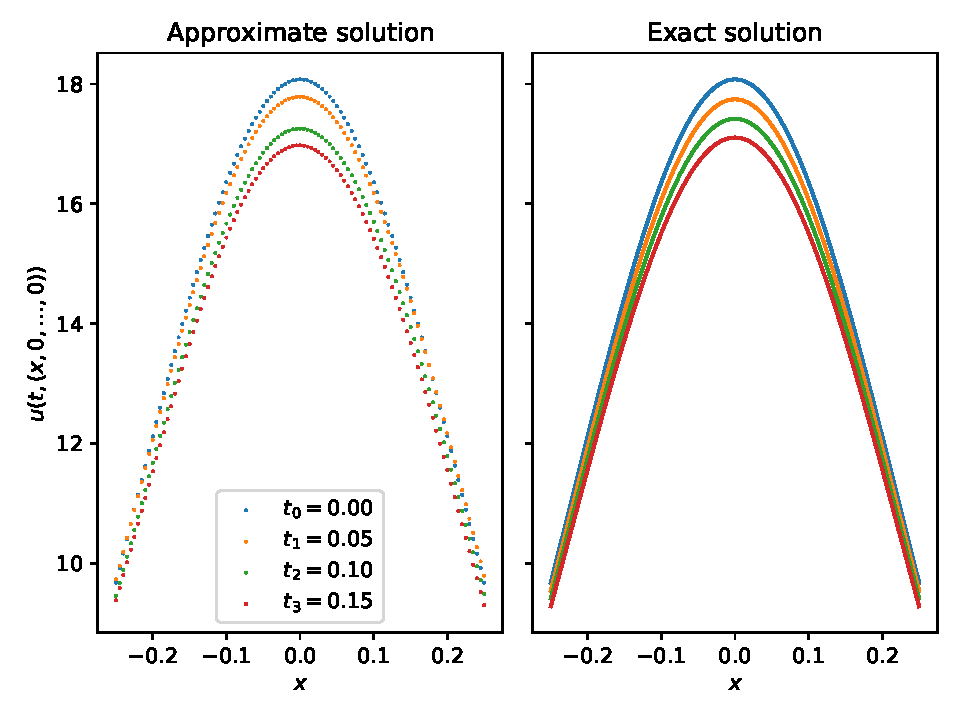
\includegraphics[width=0.8\textwidth]{hamel_5d.pdf}
	\caption{Approximate plot of $[-\nicefrac{1}{4}, \nicefrac{1}{4}] \ni x \to \bV_n^{1,0}(\theta,(x, 0, 0, \dots,0)) \in \R$ as an approximation of $[-\nicefrac{1}{4}, \nicefrac{1}{4}] \ni x \to u(t_n, (x, 0, 0, \dots,0)) \in \R$ in the case of the replicator-mutator PDEs in \eqref{eq:aniso_mutator_selector} in \Cref{subsec:aniso_mutator_selector} with $d=5$, $n \in \{ 0, 1, 2, 3 \}$, $N=10$, $T = \nicefrac{1}{2}$. On the left plot we approximately represent the machine learning approximation $[-\nicefrac{1}{4}, \nicefrac{1}{4}] \ni x \to \bV_n^{1,0}(\theta,(x, 0, 0, \dots,0)) \in \R$ and on the right plot we approximately plot the exact solution $[-\nicefrac{1}{4}, \nicefrac{1}{4}] \ni x \to u(t_n, (x, 0, 0, \dots,0)) \in \R$ in \eqref{eq:lem_aniso} in the case of the replicator-mutator PDEs in \eqref{eq:aniso_mutator_selector}.}
	\label{fig:rep_mut}
\end{figure}


\begin{lemma}\label{lem:aniso_mutator_selector}
	Let
	$d \in \N$,
	$\mathfrak{u}_1,\mathfrak{u}_2, \dots,\mathfrak{u}_d\in \R$,
	$\mathfrak{m}_1,\mathfrak{m}_2, \dots,\mathfrak{m}_d,
	\mathfrak{s}_1,\mathfrak{s}_2, \dots,\mathfrak{s}_d \in (0,\infty)$,
	let
	$a \colon \R^d \to \R$
	satisfy for every
	$x = (x_1, \dots,x_d) \in \R^d$
	that
	$a(x) = -\frac{1}{2} \sum_{i=1}^d|x_i|^2$,
	for every $i \in \{1,2,\dots,d\}$
	let
	$\mathfrak{S}_i \colon [0,\infty) \to (0,\infty)$
	and
	$\mathfrak{U}_i \colon [0,\infty) \to \R$
	satisfy for every
	$t \in [0,\infty)$
	that
	\begin{equation}\label{lem:S_U}
	\mathfrak{S}_i(t) = \mathfrak{m}_i \left[ \frac{\mathfrak{m}_i \sinh(\mathfrak{m}_i  t) + \mathfrak{s}_i \cosh(\mathfrak{m}_i t)}{\mathfrak{m}_i \cosh(\mathfrak{m}_i  t) + \mathfrak{s}_i \sinh(\mathfrak{m}_i t)}\right]\! \quad \text{and} \quad
	\mathfrak{U}_i(t) = \frac{\mathfrak{m}_i \mathfrak{u}_i}{\mathfrak{m}_i \cosh(\mathfrak{m}_i  t) + \mathfrak{s}_i \sinh(\mathfrak{m}_i t)},
	\end{equation}
	and let
	$u \colon [0,\infty) \times \R^d \to \R $
	satisfy for every
	$t \in [0,\infty)$,
	$x = (x_1,\dots,x_d)\in \R^d$
	that
	\begin{equation}\label{eq:lem_aniso}
		u(t,x) = (2\pi)^{- d/2} \left[ \prod_{ i = 1 }^d |\mathfrak{S}_i(t)|^{- 1/2} \right]     \exp \! \left(-\sum_{i = 1}^d \frac{(x_i -\mathfrak{U}_i(t) )^2}{2\mathfrak{S}_i(t)}\right).
	\end{equation}
	Then
	\begin{enumerate}[label=(\roman*)]
			\item \label{lem:it_smoothness} it holds that
			$u  \in C^{1,2}([0,\infty)\times\R^d,\R)$,
			\item \label{lem:it_u0} it holds for every
			$x = (x_1,\dots,x_d)\in \R^d$
			that
			$u(0,x) = (2\pi)^{-d/2} \big[\prod_{ i = 1 }^d |\mathfrak{s}_i|^{-1/2}\big] \exp \! \big(-\sum_{i = 1}^d \frac{(x_i - \mathfrak{u}_i )^2}{2\mathfrak{s}_i}\big)$,
			and
	    \item \label{lem:it_eq} it holds for every
			$t \in [0,\infty)$,
			$x = (x_1,\dots,x_d)\in \R^d$
			that
	    \begin{equation}
	        (\tfrac{\partial }{\partial t}u) (t,x) = u(t,x)\!  \left(a(x) - \int_{\R^d} u(t,{\textbf x})\, a({\textbf x}) \, d{\textbf x} \right) + \smallsum_{i=1}^{d} \frac{1}{2} (\mathfrak{m}_i)^2(\tfrac{\partial^2 }{\partial x_i^2} u) (t,x).
	        \label{eq:lemma_replicator_mutator}
	    \end{equation}

	\end{enumerate}
\end{lemma}

\begin{proof}[Proof of \Cref{lem:aniso_mutator_selector}]
	First, note that the fact for every
	$i \in \{1,2,\dots,d\}$
	it holds that
	$\mathfrak{S}_i \in C^{\infty}([0,\infty),(0,\infty))$,
	the fact for every
	$i \in \{1,2,\dots,d\}$
	it holds that
	$\mathfrak{U}_i \in C^{\infty}([0,\infty),\R) $,
	and \eqref{eq:lem_aniso}
	establish item \eqref{lem:it_smoothness}.
	Moreover, observe that the fact for every
	$i \in \{1,2,\dots,d\}$
	it holds that
	$\mathfrak{S}_i(0) = \mathfrak{s}_i$,
	the fact for every
	$i \in \{1,2,\dots,d\}$
	it holds that
	$\mathfrak{U}_i(0) = \mathfrak{u}_i$,
	and
	\eqref{lem:S_U}
	establish  item \eqref{lem:it_u0}.
	Next note that \eqref{eq:lem_aniso} ensures that for every
	$t \in [0,\infty)$,
	$x = (x_1,\dots,x_d)\in \R^d$
	it holds that
	\begin{equation}\label{eq:lem_u}
		u(t,x) = \prod_{i=1}^d \left[ (2\pi    \mathfrak{S}_i(t))^{-1/2}    \exp \! \left( - \frac{(x_i -\mathfrak{U}_i(t) )^2}{2\mathfrak{S}_i(t)}\right) \right].
	\end{equation}
	The product rule hence implies that for every
	$t \in [0,\infty)$,
	$x = (x_1,\dots,x_d)\in \R^d$
	it holds that
	\begin{equation}
	\begin{split}
			&(\tfrac{\partial }{\partial t}u) (t,x)  \\
			& = \frac{\partial}{\partial t} \left(\prod_{i=1}^d \left[ (2\pi   \mathfrak{S}_i(t))^{-1/2}  \exp \left( - \frac{(x_i -\mathfrak{U}_i(t) )^2}{2\mathfrak{S}_i(t)}\right) \right] \right)\\
			& = \sum_{i=1}^d \Bigg[  \bigg[ \prod\nolimits_{ j \in \{ 1,\dots,d \} \backslash i} \left( (2\pi \mathfrak{S}_j(t))^{-1/2} \exp \! \left( - \frac{(x_j -\mathfrak{U}_j(t) )^2}{2\mathfrak{S}_j(t)}\right) \right)\bigg]\\
			&\quad \cdot \left[ \frac{\partial}{\partial t} \left( (2\pi   \mathfrak{S}_i(t))^{-1/2}   \exp \! \left(- \frac{(x_i -\mathfrak{U}_i(t) )^2}{2\mathfrak{S}_i(t)}\right) \right)  \right] \Bigg].
	\end{split} 
	\end{equation}
	The chain rule and \eqref{eq:lem_u} hence ensure that for every
	$t \in [0,\infty)$,
	$x = (x_1,\dots,x_d)\in \R^d$
	it holds that
	\begin{equation}\label{lem:derivatives1}
		\begin{split}
				&(\tfrac{\partial }{\partial t}u) (t,x)  \\
				& = \sum_{i=1}^d \Bigg[  \bigg[ \prod\nolimits_{ j \in \{ 1,\dots,d \} \backslash i} \left( (2\pi \mathfrak{S}_j(t))^{-1/2} \exp \! \left( - \frac{(x_j -\mathfrak{U}_j(t) )^2}{2\mathfrak{S}_j(t)}\right) \right)\bigg]\\
				&\quad \cdot \bigg[\left( \frac{\partial}{\partial t} \left( (2\pi   \mathfrak{S}_i(t))^{-1/2} \right) \right) \left( \exp \! \left(- \frac{(x_i -\mathfrak{U}_i(t) )^2}{2\mathfrak{S}_i(t)}\right) \right) \\
				&\quad + \left( (2\pi   \mathfrak{S}_i(t))^{-1/2} \right) \left( \frac{\partial}{\partial t}  \left( - \frac{(x_i -\mathfrak{U}_i(t) )^2}{2\mathfrak{S}_i(t)} \right) \right) \left(\exp \! \left(- \frac{(x_i -\mathfrak{U}_i(t) )^2}{2\mathfrak{S}_i(t)}\right) \right)  \bigg] \Bigg] \\
				&=  \sum_{i=1}^d \Bigg[  \bigg[ \prod\nolimits_{ j \in \{ 1, \dots,d \} \backslash i} \left( (2\pi \mathfrak{S}_j(t))^{-1/2} \exp \! \left( - \frac{(x_j -\mathfrak{U}_j(t) )^2}{2\mathfrak{S}_j(t)}\right) \right)\bigg]\\
				&\quad \cdot \bigg[   - \left( (2\pi  \mathfrak{S}_i(t))^{-1/2}\right)\frac{\left( \tfrac{\partial }{\partial t}\mathfrak{S}_i) (t)\right)}{2\mathfrak{S}_i(t)} \exp \! \left(- \frac{(x_i -\mathfrak{U}_i(t) )^2}{2\mathfrak{S}_i(t)}\right) \\
				&\quad + \left( (2\pi  \mathfrak{S}_i(t))^{-1/2}\right) \bigg(  \frac{ 2(\tfrac{\partial }{\partial t}\mathfrak{U}_i)(t)(x_i-\mathfrak{U_i}(t))}{2\mathfrak{S}_i(t)} \\
				&\quad  + \frac{(x_i-\mathfrak{U}_i(t))^2 (\tfrac{\partial }{\partial t}\mathfrak{S}_i)(t)}{2|\mathfrak{S}_i(t)|^{2}} \bigg) \exp \! \left(- \frac{(x_i -\mathfrak{U}_i(t) )^2}{2\mathfrak{S}_i(t)}\right) \bigg] \Bigg] \\
				& = u(t,x) \Bigg[ \sum_{i=1}^d\left( \frac{-(\tfrac{\partial }{\partial t}\mathfrak{S}_i) (t)}{2\mathfrak{S}_i(t)} +
					\frac{ 2\mathfrak{S}_i(t) (\tfrac{\partial }{\partial t}\mathfrak{U}_i)(t)(x_i-\mathfrak{U_i}(t)) + (x_i-\mathfrak{U}_i(t))^2 (\tfrac{\partial }{\partial t}\mathfrak{S}_i)(t)}{2|\mathfrak{S}_i(t)|^{2}}\right) \Bigg].
		\end{split} 
	\end{equation}
	Moreover, observe that \eqref{lem:S_U}, the chain rule, and the product rule ensure that for every
	$i \in \{1, \dots,d\}$,
	$t \in [0,\infty)$
	it holds that
	\begin{equation}
		\begin{aligned}
			(\tfrac{\partial }{\partial t}\mathfrak{U}_i)(t) &= \frac{\partial }{\partial t} \left( \frac{\mathfrak{m}_i \mathfrak{u}_i}{\mathfrak{m}_i \cosh(\mathfrak{m}_i  t) + \mathfrak{s}_i \sinh(\mathfrak{m}_i t)} \right)\\
			&= - |\mathfrak{m}_i|^2 \mathfrak{u}_i \left[ \frac{\mathfrak{m}_i \sinh(\mathfrak{m}_i  t) + \mathfrak{s}_i \cosh(\mathfrak{m}_i t)}{\left[ \mathfrak{m}_i \cosh(\mathfrak{m}_i  t) + \mathfrak{s}_i \sinh(\mathfrak{m}_i t)\right]^2} \right]\\
			&= - \mathfrak{S}_i(t)    \mathfrak{U}_i(t) 
		\end{aligned}
	\end{equation}
	and
	\begin{equation}
		\begin{aligned}
			(\tfrac{\partial }{\partial t}\mathfrak{S}_i)(t) &= \frac{\partial }{\partial t} \left( \mathfrak{m}_i \left[ \frac{\mathfrak{m}_i \sinh(\mathfrak{m}_i  t) + \mathfrak{s}_i \cosh(\mathfrak{m}_i t)}{\mathfrak{m}_i \cosh(\mathfrak{m}_i  t) + \mathfrak{s}_i \sinh(\mathfrak{m}_i t)}\right]\right) \\
			&= |\mathfrak{m}_i|^2 \left[ \frac{\mathfrak{m}_i \cosh(\mathfrak{m}_i  t) + \mathfrak{s}_i \sinh(\mathfrak{m}_i t)}{\mathfrak{m}_i \cosh(\mathfrak{m}_i  t) + \mathfrak{s}_i \sinh(\mathfrak{m}_i t)}\right] - |\mathfrak{m}_i|^2\left[ \frac{\mathfrak{m}_i \sinh(\mathfrak{m}_i  t) + \mathfrak{s}_i \cosh(\mathfrak{m}_i t)}{ \mathfrak{m}_i \cosh(\mathfrak{m}_i  t) + \mathfrak{s}_i \sinh(\mathfrak{m}_i t)} \right]^2\\
			&= |\mathfrak{m}_i|^2  - |\mathfrak{S}_i(t)|^2.
		\end{aligned}
	\end{equation}
	%
	Combining this with \eqref{lem:derivatives1} yields that for every
	$i \in \{1, \dots,d\}$,
	$t \in [0,\infty)$
	it holds that
	\begin{equation}\label{lem:derivatives1*}
		\begin{split}
				&(\tfrac{\partial }{\partial t}u) (t,x)  \\
				&= \frac{u(t,x)}{2} \Bigg[ \sum_{i=1}^d\Bigg[ \frac{-\big[|\mathfrak{m}_i|^2  - |\mathfrak{S}_i(t)|^2\big]}{\mathfrak{S}_i(t)} \\
				&\quad + \frac{ 2|\mathfrak{S}_i(t)|^2  \mathfrak{U}_i(t) (\mathfrak{U_i}(t) - x_i) + (x_i-\mathfrak{U}_i(t))^2 (|\mathfrak{m}_i|^2  - |\mathfrak{S}_i(t)|^2)}{|\mathfrak{S}_i(t)|^{2}}\Bigg] \Bigg]\\
				&= \frac{u(t,x)}{2} \Bigg[ \sum_{i=1}^d\Bigg[ |\mathfrak{m}_i|^2  \left( \bigg(\frac{x_i - \mathfrak{U}_i(t)}{\mathfrak{S}_i(t)}\bigg)^{\!2} - \frac{1}{\mathfrak{S}_i(t)} \right) \\
				&\quad + \mathfrak{S}_i(t) + 2\left(|\mathfrak{U}_i(t)|^2 - \mathfrak{U}_i(t)\, x_i\right) - \left(|x_i|^2 -2 \mathfrak{U}_i(t) \, x_i + |\mathfrak{U}_i(t)|^2 \right)  \Bigg] \Bigg]\\
				&= \frac{u(t,x)}{2} \left[ \sum_{i=1}^d \left[  |\mathfrak{m}_i|^2  \left( \bigg(\frac{x_i - \mathfrak{U}_i(t)}{\mathfrak{S}_i(t)}\bigg)^{\!2} - \frac{1}{\mathfrak{S}_i(t)} \right) + \mathfrak{S}_i(t) + |\mathfrak{U}_i(t)|^2 - |x_i|^2 \right]\right].
		\end{split}
	\end{equation}
	%
	Moreover, note that \eqref{eq:lem_u} and the product rule demonstrate that for every
	$i \in \{1, \dots,d\}$,
	$t \in [0,\infty)$,
	$x = (x_1, \dots,x_d)\in \R^d$
	it holds that 
	\begin{equation}
		\begin{split}
			&( \tfrac{\partial }{\partial x_i} u)(t,x)\\
			&=  \frac{\partial }{\partial x_i}  
			\left[\prod_{j = 1}^d\left[(2\pi   \mathfrak{S}_j(t))^{-1/2}   \exp \! \left( - \frac{(x_j -\mathfrak{U}_j(t) )^2}{2\mathfrak{S}_j(t)}\right) \right] \right]\\
			&= \left[ \frac{\partial }{\partial x_i} 
				\left[(2\pi   \mathfrak{S}_i(t))^{-1/2}   \exp \! \left( - \frac{(x_i -\mathfrak{U}_i(t) )^2}{2\mathfrak{S}_i(t)} \right) \right] \right]\\
				&\quad \cdot \Bigg[\prod_{ j \in \{ 1, \dots,d \} \backslash i} \left[ (2\pi   \mathfrak{S}_j(t))^{-1/2}   \exp \! \left( - \frac{(x_j -\mathfrak{U}_j(t) )^2}{2\mathfrak{S}_j(t)} \right) \right] \Bigg]\\
			&= - u(t,x) \bigg( \frac{x_i - \mathfrak{U}_i(t)}{\mathfrak{S}_i(t)} \bigg) = u(t,x) \bigg( \frac{\mathfrak{U}_i(t) - x_i }{\mathfrak{S}_i(t)} \bigg).
		\end{split}
	\end{equation}
	The product rule and \eqref{eq:lem_u} therefore assure that for every
	$i \in \{1, \dots,d\}$,
	$t \in [0,\infty)$,
	$x = (x_1, \dots,x_d)\in \R^d$
	it holds that 
	\begin{equation}
		\begin{split}
			&( \tfrac{\partial^2 }{\partial x_i^2} u )(t,x) = \frac{\partial }{\partial x_i} \left(u(t,x) \bigg( \frac{ \mathfrak{U}_i(t) - x_i}{\mathfrak{S}_i(t)} \bigg)\right)\\
			&= u(t,x) \left[ \bigg(\frac{\mathfrak{U}_i(t) - x_i}{\mathfrak{S}_i(t)}\bigg)^{\!2} - \frac{1}{\mathfrak{S}_i(t)} \right] = u(t,x) \left[ \bigg(\frac{x_i - \mathfrak{U}_i(t)}{\mathfrak{S}_i(t)}\bigg)^{\!2} - \frac{1}{\mathfrak{S}_i(t)} \right].
		\end{split}
	\end{equation}
	Hence, we obtain that for every
	$t \in [0,\infty)$,
	$x = (x_1, \dots,x_d)\in \R^d$
	it holds that 
	\begin{equation}\label{lem:derivatives2}
		\begin{split}
			&\left[ \sum_{i=1}^d \left[ \left( \tfrac{1}{2} |\mathfrak{m}_i|^2\right)(\tfrac{\partial^2 }{\partial x_i^2} u) (t,x) \right] \right] 
			= \frac{u(t,x)}{2} \left[ \sum_{i=1}^d \left[ |\mathfrak{m}_i|^2 \left( \bigg(\frac{x_i - \mathfrak{U}_i(t)}{\mathfrak{S}_i(t)}\bigg)^{\!2} - \frac{1}{\mathfrak{S}_i(t)} \right)\right]\right].
		\end{split}
	\end{equation}
	Next observe that \eqref{eq:lem_u} ensures that for every
	$t \in [0,\infty)$,
	$x = (x_1, \dots,x_d)\in \R^d$
	it holds that
	\begin{equation}
		\begin{split}
			&u(t,x)\left( a(x) - \int_{\R^d} u(t,{\textbf x})\, a({\textbf x}) \, d{\textbf x} \right) \\
			&= u(t,x) \left(\left[ - \tfrac{1}{2} \right] \left[\sum_{i=1}^d |x_i|^2 \right] - \int_{\R^d} \left[ - \tfrac{1}{2} \right] \left[ \sum_{i=1}^d |{\textbf x}_i|^2 \right] u(t,{\textbf x}) \, d {\textbf x} \right)\\
			&= \frac{u(t,x)}{2} \Biggl( - \left[\sum_{i=1}^d |x_i|^2 \right] \\
			&\quad + \sum_{i=1}^d \bigg[ \int_\R \left( |{\textbf x}_i|^2 \, (2\pi    \mathfrak{S}_i(t))^{-1/2}    \exp \! \left( - \frac{({ \textbf x}_i -\mathfrak{U}_i(t) )^2}{2\mathfrak{S}_i(t)}\right) \right) d{\textbf x}_i  \\
			&\quad \cdot \bigg(\prod\nolimits_{ j \in \{ 1, \dots,d \} \backslash i} \int_\R \left((2\pi    \mathfrak{S}_j(t))^{-1/2}    \exp \! \left( - \frac{({\textbf x}_j -\mathfrak{U}_j(t) )^2}{2\mathfrak{S}_j(t)}\right) \right) d{\textbf x_j} \bigg) \bigg] \Biggr).
			\end{split}
		\end{equation}
	This and the fact for every
	$i \in \{1, \dots, d\}$,
	$t \in [0,\infty)$
	it holds that
	\begin{equation}
		\int_\R \left( (2\pi    \mathfrak{S}_i(t))^{-1/2}    \exp \! \left( - \frac{( x -\mathfrak{U}_i(t) )^2}{2\mathfrak{S}_i(t)}\right) \right) d x  = 1
	\end{equation}
	imply that for every
	$t \in [0,\infty)$,
	$x = (x_1, \dots,x_d)\in \R^d$
	it holds that 
	\begin{equation}\label{lem:derivatives4}
		\begin{split}
			&u(t,x)\left( a(x) - \int_{\R^d} u(t,{\textbf x})\, a({\textbf x}) \, d{\textbf x} \right) \\
			&= \frac{u(t,x)}{2} \Biggl(\sum_{i=1}^d \left[- |x_i|^2 + \int_\R \left( |{\textbf x}_i|^2 \, (2\pi    \mathfrak{S}_i(t))^{-1/2}    \exp \! \left( - \frac{({ \textbf x}_i -\mathfrak{U}_i(t) )^2}{2\mathfrak{S}_i(t)}\right) \right) d{\textbf x}_i \right]\Bigg).
		\end{split}
	\end{equation}
	Next observe that the integral transformation theorem demonstrates that for every
	$i \in \{1, \dots,d\}$,
	$t \in [0,\infty)$
	it holds that
	\begin{equation}
		\begin{aligned}
			&\int_\R \left(  x^2 \left[ (2\pi    \mathfrak{S}_i(t))^{-1/2}    \exp \! \left( - \frac{( x -\mathfrak{U}_i(t) )^2}{2\mathfrak{S}_i(t)}\right) \right] \right) d x \\
			&= \int_\R \left(  (x + \mathfrak{U}_i(t))^2 \left[ (2\pi    \mathfrak{S}_i(t))^{-1/2}    \exp \! \left( - \frac{x^2}{2\mathfrak{S}_i(t)}\right) \right] \right) d x\\
			&= \int_\R \left(  x ^2 \left[ (2\pi    \mathfrak{S}_i(t))^{-1/2}    \exp \! \left( - \frac{x^2}{2\mathfrak{S}_i(t)}\right) \right] \right) d x \\
			&\quad + \int_\R \left(  |\mathfrak{U}_i(t)|^2 \left[ (2\pi    \mathfrak{S}_i(t))^{-1/2}    \exp \! \left( - \frac{x^2}{2\mathfrak{S}_i(t)}\right) \right] \right) d x\\
			&=\mathfrak{S}_i(t) + |\mathfrak{U}_i(t)|^2.
		\end{aligned}
	\end{equation}
	Combining this with \eqref{lem:derivatives4} ensures that for every
	$t \in [0,\infty)$,
	$x = (x_1, \dots,x_d)\in \R^d$
	it holds that 
	\begin{equation}\label{lem:derivatives3}
		\begin{split}
			&u(t,x)\left( a(x) - \int_{\R^d} u(t,{\textbf x})\, a({\textbf x}) \, d{\textbf x} \right) = \frac{u(t,x)}{2} \left[ \sum_{i=1}^d \left( \mathfrak{S}_i(t) + |\mathfrak{U}_i(t)|^2 - |x_i|^2 \right) \right].
		\end{split}
	\end{equation}
	This and \eqref{lem:derivatives2} demonstrate that for every
	$t \in [0,\infty)$,
	$x = (x_1, \dots,x_d)\in \R^d$
	it holds that
	\begin{equation}
		\begin{aligned}
			& u(t,x)\left(a(x) - \int_{D} u(t,{\textbf x})\, a({\textbf x}) \, d{\textbf x} \right) + \smallsum_{i=1}^{d} \frac{1}{2} |\mathfrak{m}_i|^2 (\tfrac{\partial^2 }{\partial x_i^2} u) (t,x) \\
			&= \frac{u(t,x)}{2} \left[ \sum_{i=1}^d \left[  |\mathfrak{m}_i|^2  \left( \bigg(\frac{x_i - \mathfrak{U}_i(t)}{\mathfrak{S}_i(t)}\bigg)^{\!2} - \frac{1}{\mathfrak{S}_i(t)} \right) + \mathfrak{S}_i(t) + |\mathfrak{U}_i(t)|^2 - |x_i|^2 \right]\right].
		\end{aligned}
	\end{equation}
	%
	Combining this with \eqref{lem:derivatives1*} establishes item \eqref{lem:it_eq}. This completes the proof of \Cref{lem:aniso_mutator_selector}.
\end{proof}

\subsection{Allen--Cahn PDEs with conservation of mass}
\label{subsec:allen_cahn}
%
In this subsection we use the machine learning-based approximation method in \Cref{frame:adam}
to approximately calculate the solutions of certain Allen--Cahn PDEs with cubic nonlinearity, conservation of mass and no-flux boundary conditions (cf., e.g., Rubinstein \& Sternberg \cite{RUBINSTEIN1992}).

Assume \Cref{frame:adam}, 
let
$\epsilon = \tfrac{1}{10}$,
assume that
$d\in\{1,2,5,10\}$,
$\D = [0,1]^d$,
$T\in\{\nicefrac{1}{5},\nicefrac{1}{2},1\}$,
$N=10$,
$K_1 = K_2 = \ldots = K_N= 1$, and
$M_1 = M_2 = \ldots = M_N = 400$,
%$\varepsilon=10^{-8}$,
assume that 
$\xi^{n,m,j}, n, m, j \in \N$
are independent $\mathcal{U}_{D}$-distributed random variables,
assume for every 
$m \in \N$
that
$\gamma_m =10^{-2}$,
and
assume for every 
$s,t \in [0,T]$, 
$v,x,{\textbf x},z, {\textbf z} \in \R^d$, 
$y,{\textbf y} \in \R$,
$A \in \mathcal{B}(D)$
that
$\nu_x(A) = \int_A d{\textbf x}$,
$g(x)= \exp (-\tfrac{1}{2}\|x\|^2)$,
$\mu(x)=(0, \dots, 0)$,
$\sigma(x) v = \sqrt{2} v$, 
$f(t,x,{\textbf x},y,{\textbf y}, z, {\textbf z})=  y - y^3 - \left( {\textbf y} - {\textbf y}^3\right)$, and
\begin{equation}
	H(t,s,x,v) = R(x,x+\mu(x)(t-s)+\sigma(x)v)
\end{equation}
(cf.\ \eqref{Y-algo-spez} and \eqref{eq:FormalXapprox}).
The solution $u\colon[0,T]\times \R^d \to \R$ of the PDE in \eqref{eq:PDE-Examples} then satisfies that for every
$t\in [0,T]$, $x\in\R^d$ it holds that $u(0,x)=\exp (-\tfrac{1}{2}\|x\|^2)$ and
%
\begin{equation}
 (\tfrac{\partial}{\partial t}u)(t,x)
 =
 \tfrac{\epsilon^2}{2} (\Delta_x u)(t,x) + u(t,x) - [u(t,x)]^3 - \int_{[0,1]^d} \left(u(t,{\textbf x}) - [u(t,{\textbf x})]^3 \right) \!d{\textbf x} .
 \label{eq:allen_cahn}
\end{equation}
%
%
In \Cref{table:allen_cahn}
we use the machine learning-based approximation method
in \Cref{frame:adam}
to approximately calculate
the mean of %$\Theta^{(1)}_m$,
$
\bV^{1,0}_N(\Theta^N_M,x)
$,
the standard deviation of %$\Theta^{(1)}_m$,
$
\bV^{1,0}_N(\Theta^N_M,x)
$,
the $ L^1 $-approximation error associated to %$\Theta^{(1)}_m$,
$
\bV^{1,0}_N(\Theta^N_M,x)
$,
the uncorrected sample standard deviation of the approximation error associated to %$ \Theta^{(1)}_m $,
$
\bV^{1,0}_N(\Theta^N_M,x)
$,
%the mean of the loss function associated to $\Theta_m$,
%the standard deviation of the loss function associated to $\Theta_m$,
and the average runtime in seconds needed for calculating one realization of $
\bV^{1,0}_N(\Theta^N_M,x)
$
%
based on $5$ independent realizations (5 independent runs).
%
The reference value, which is used as an approximation for the unknown value $u(T,0,0,\ldots,0)$ of the exact solution of \eqref{eq:allen_cahn}, has been calculated through the multilevel Picard approximation method for non-local nonlinear PDEs in \Cref{frame:mlpsetting} (see \Cref{exampleMLP:allen_cahn}).

\begin{table}% temporary results to be updated, waiting for simulations 
	\begin{center}
		\resizebox{\textwidth}{!}{\begin{tabular}{|c|c|c|c|c|c|c|c|c|}
			\hline
			$ d $ & $T$ & $N$ & Mean & Std.\ dev.\ & Ref.\ value & $L^1$-error & Std.\ dev.\ error & avg.\ runtime\\
			\hline
			1 & \nicefrac{1}{5} & 10 & 1.1357852 & 0.00004031 & 1.1329060 & 0.0025414 & 0.0000356 & 11.403\\
			2 & \nicefrac{1}{5} & 10 & 1.1667370 & 0.00011471 & 1.1629940 & 0.0032184 & 0.0000986 & 11.351\\
			5 & \nicefrac{1}{5} & 10 & 1.1704630 & 0.00005095 & 1.1664700 & 0.0034231 & 0.0000437 & 11.137\\
			10 & \nicefrac{1}{5} & 10 & 1.1650314 & 0.00004317 & 1.1609480 & 0.0035173 & 0.0000372 & 11.179\\
			\hline
			1 & \nicefrac{1}{2} & 10 & 1.3500632 & 0.00009184 & 1.3409300 & 0.0068111 & 0.0000685 & 11.118\\
			2 & \nicefrac{1}{2} & 10 & 1.4364596 & 0.00004400 & 1.4269380 & 0.0066727 & 0.0000308 & 11.215\\
			5 & \nicefrac{1}{2} & 10 & 1.4472808 & 0.00006241 & 1.4338880 & 0.0093402 & 0.0000435 & 11.199\\
			10 & \nicefrac{1}{2} & 10 & 1.4325428 & 0.00006902 & 1.4209860 & 0.0081329 & 0.0000486 & 11.174\\
			\hline
			1 & 1 & 10 & 1.7087326 & 0.00020741 & 1.6880340 & 0.0122620 & 0.0001229 & 11.070\\
			2 & 1 & 10 & 1.8962484 & 0.00006563 & 1.8653440 & 0.0165677 & 0.0000352 & 11.076\\
			5 & 1 & 10 & 1.9221128 & 0.00008683 & 1.8889600 & 0.0175508 & 0.0000460 & 11.082\\
			10 & 1 & 10 & 1.8934832 & 0.00009063 & 1.8588340 & 0.0186403 & 0.0000488 & 11.148\\
			\hline
		\end{tabular}}
	\end{center}
	\caption{Numerical simulations for the approximation method in \Cref{def:general_algorithm} in the case of the Allen--Cahn PDEs with conservation of mass in \eqref{eq:allen_cahn} in \Cref{subsec:allen_cahn}.
	\label{table:allen_cahn}}
\end{table}